\documentclass{beamer}

\usepackage{beamerthemesplit}

\setbeamertemplate{footline}[page number]{}

\setbeamertemplate{navigation symbols}{}

\title{Bayes Seminar: Part I}
\author{John Myles White}
\date{\today}

\begin{document}

\frame{\titlepage}

\frame
{
  Statistical theory, minimally, tries to answer two questions:
  \begin{itemize}
    \item{What can we learn from experience?}
    \item{How should we best learn from experience?}
  \end{itemize}
}

\frame
{
  Bayesian statistical theory answers one additional question:
  \begin{itemize}
    \item{How should we represent the knowledge we gain from experience?}
  \end{itemize}
}

\frame
{
  \begin{itemize}
    \item{Since Hume, we've known that induction is problematic}
    \item{How do we use experiences that are not perfectly informative?}
  \end{itemize}
}

\frame
{
  A motivating example:
  \begin{itemize}
    \item{Imagine that you've gone to a new restaurant for the first time}
    \item{A mistake is made with your order}
    \item{Do you conclude that a mistake is made with every order?}
  \end{itemize}
}

\frame
{
  \begin{itemize}
    \item{Most people will not reach this conclusion}
    \item{Some statistical methods will reach this conclusion}
    \item{We'd like to decide what is the \emph{right} conclusion to draw}
    \item{How can we formalize the situation for mathematical analysis?}
  \end{itemize}
}

\frame
{
  \begin{itemize}
    \item<1->{We assume that each order either has a mistake or doesn't}
    \item<2->{We encode a mistake as a binary variable that takes on values of 0 or 1}
    \item<3->{We assume that this binary variable is a random variable with a probability distribution over $\{0, 1\}$}
    \item<4->{We assume that each separate order is an independent instantiation of this random variable}
  \end{itemize}
}

\frame
{
  \begin{itemize}
    \item{Those assumptions are the core elements of most probabilistic models}
    \item{Having made them, we can provide a formal analysis}
  \end{itemize}
}

\frame
{
  \begin{itemize}
    \item{Each order's accuracy is modeled as a Bernoulli variable}
    \item{$n$ orders taken together are a binomial variable}
    \item{Either model has exactly one unknown parameter: $p$, the probability of a mistake}
    \item{We want to estimate this parameter}
  \end{itemize}
}

\frame
{
 \begin{itemize}
   \item{In this context, we've answered the question of what we can learn}
   \item{$p$ is all that we can learn}
   \item{We therefore only have to ask how to learn about $p$ and how to represent what we learn}
 \end{itemize}
}

\frame
{
 Some representations of $p$:
 \begin{itemize}
   \item{Point estimation: our knowledge of $p$ is a single value $\hat{p}$}
   \item{Interval estimation: our knowledge of $p$ is a range, $[\hat{p}_{l}, \hat{p}_{u}]$}
   \item{Bayesian estimation: our knowledge of $p$ is a probability distribution over $\hat{p}$'s}
 \end{itemize}
}

\frame
{
 Some estimates given one order:
 \begin{itemize}
   \item{Point Estimate: $\hat{p} = 1$ (MLE)}
   \item{Interval Estimate: $[\hat{p}_{l}, \hat{p}_{u}]$ = [0.025, 1.000] (95\% CI)}
   \item{Bayesian Estimate:}
   \begin{center}
     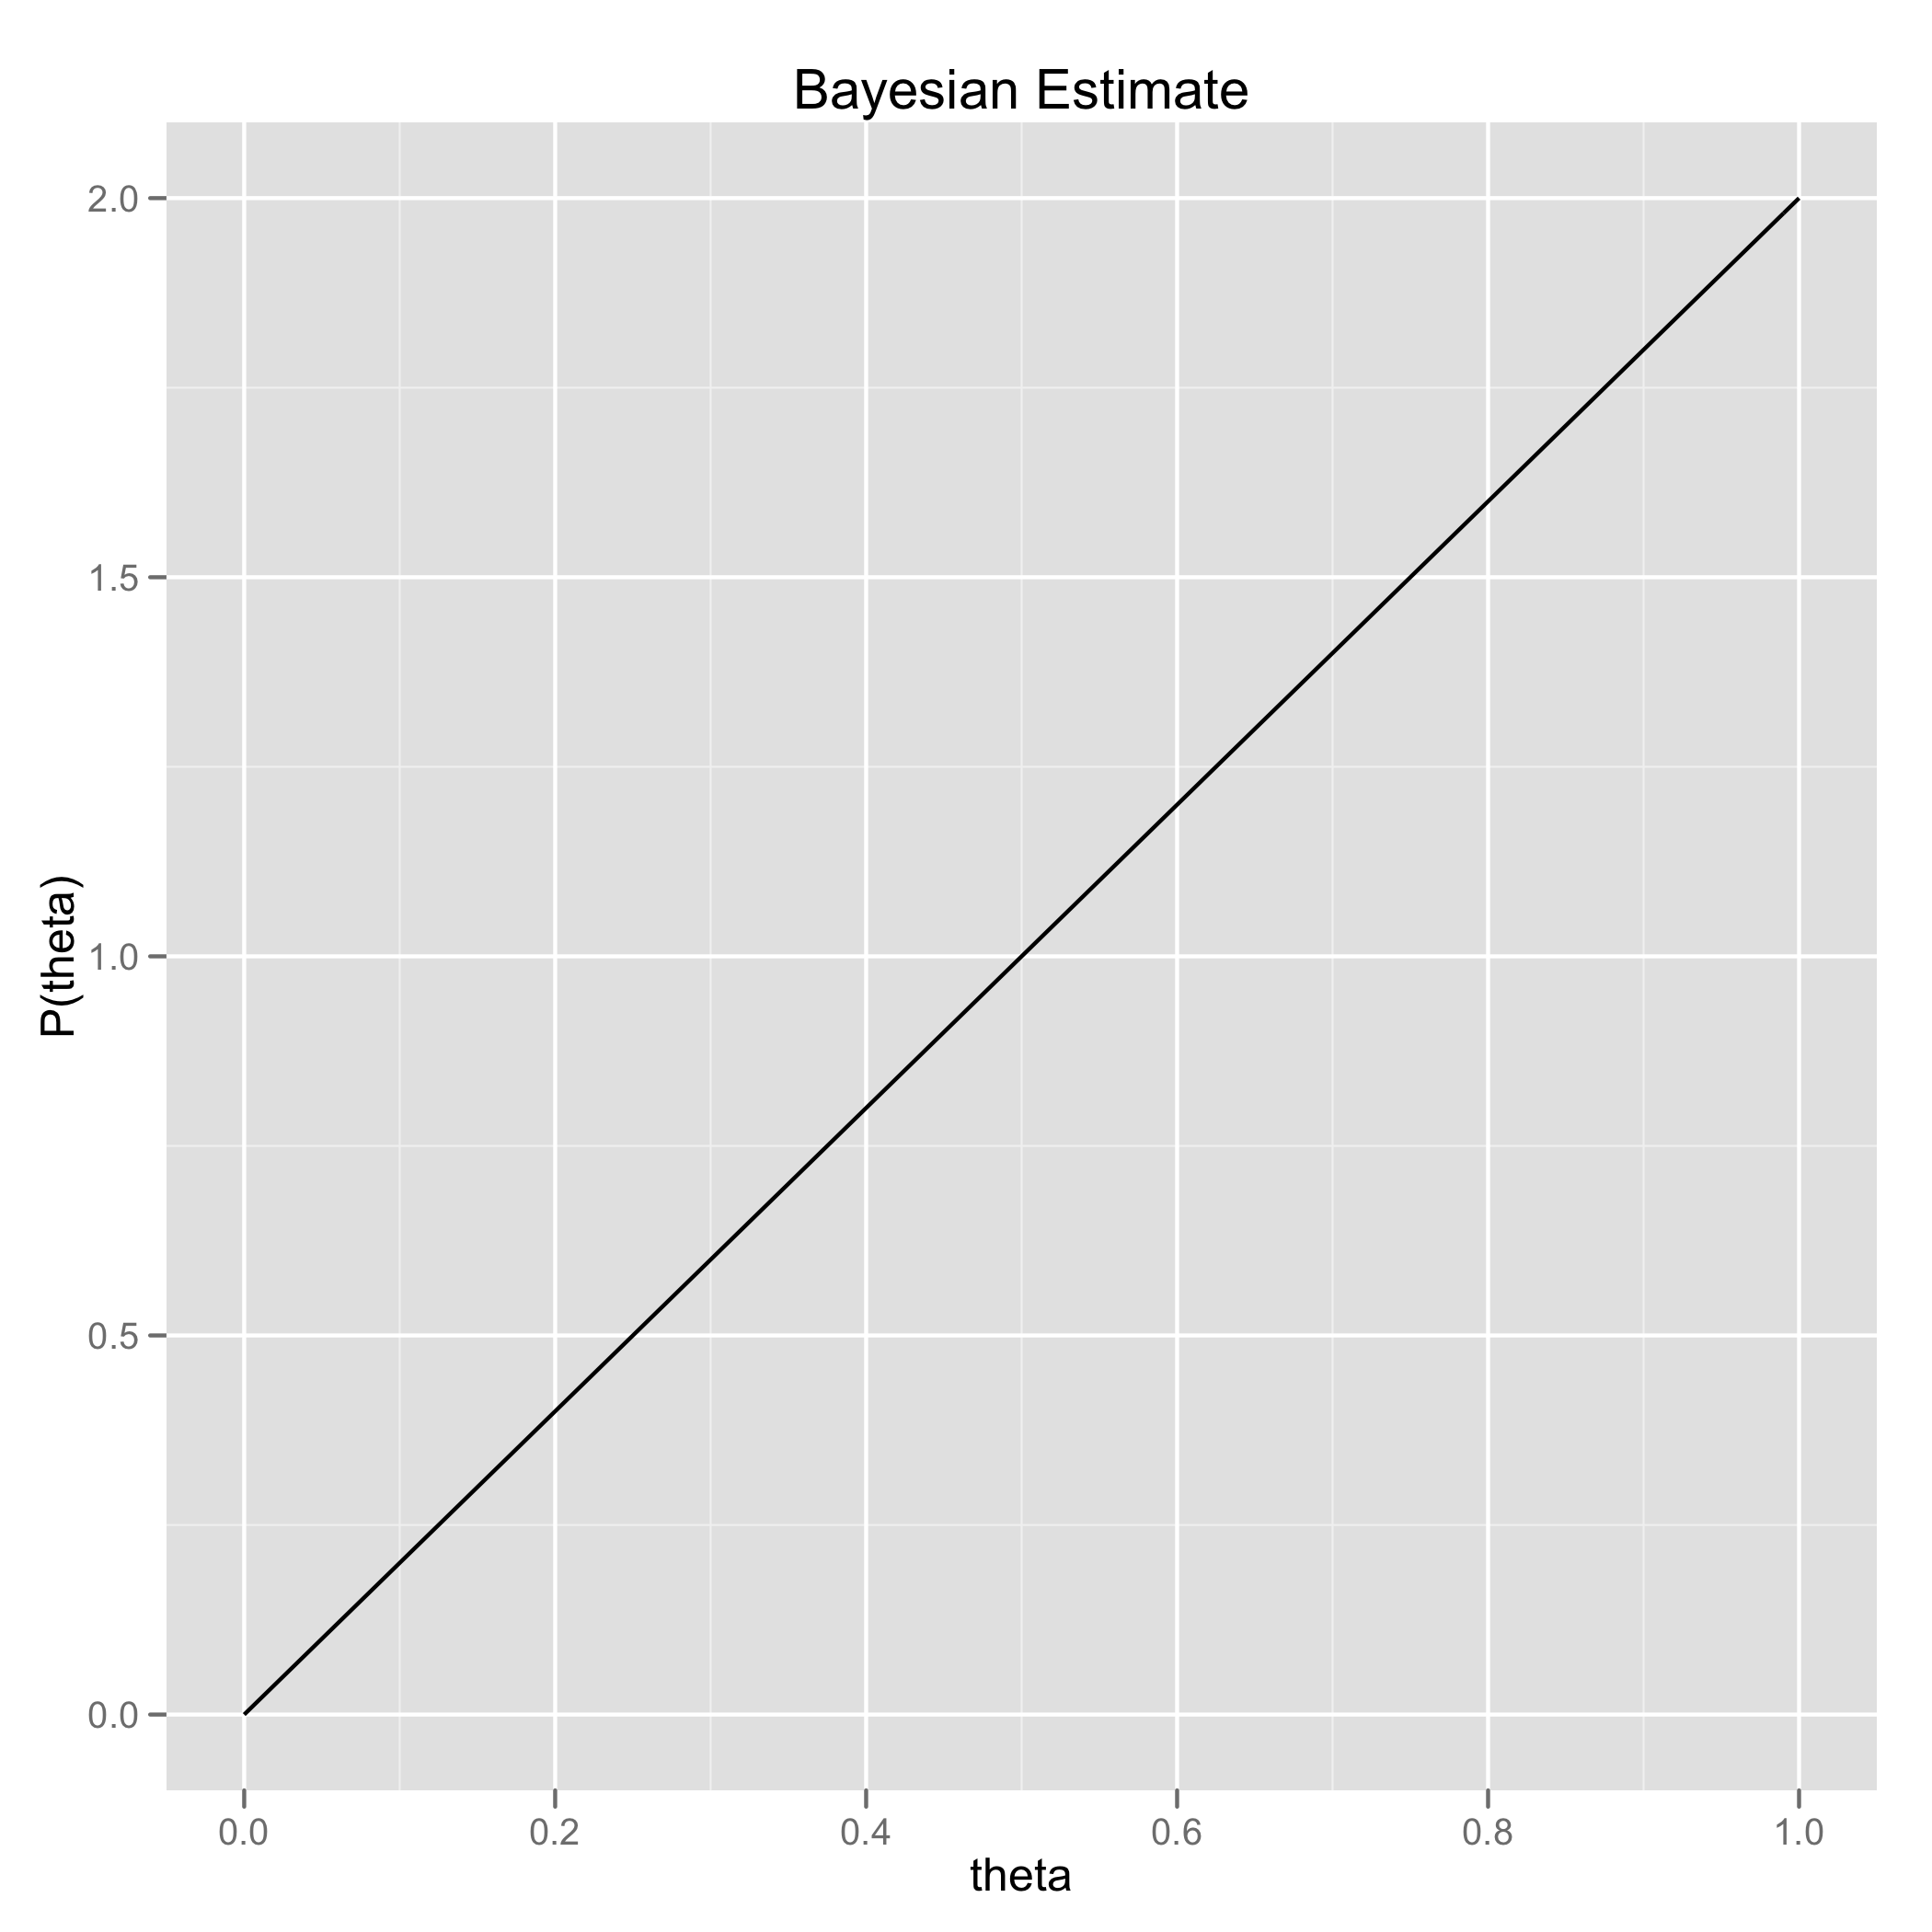
\includegraphics[scale = 0.075]{sample_beta.png}
    \end{center}
 \end{itemize}
}

\frame
{
  \begin{itemize}
    \item{Throughout this seminar I'm going to focus on Bayesian estimation}
    \item{I'll contrast it with point and interval estimation}
  \end{itemize}
}

\frame
{
  Generalizing our example:
  \begin{itemize}
    \item{We have a data set, $D$, of $n$ data points: $x_1, x_2, \ldots, x_n$}
    \item{We have a probabilistic model that generates data sets}
    \item{We write the probability of a data set as $p(D) = p(x_1, x_2, \ldots, x_n)$}
    \item{In this seminar, every model will be defined by a finite number of parameters}
    \item{Instead of the single parameter, $p$, we'll have a list of parameters, $\theta$}
    \item{We then write $p(D | \theta)$}
  \end{itemize}
}

\frame
{
  \begin{itemize}
    \item{If our data set is fixed, we can treat $p(D | \theta)$ as a function of $\theta$}
    \item{We'll sometimes write $L(\theta; D)$ to describe this function}
    \item{This function is called the likelihood function}
    \item{$L$ tells us the probability of seeing any specific data set if the parameters of the model were set to $\theta$}
  \end{itemize}
}

\frame
{
  Simplifying the likelihood function:
  \begin{itemize}
    \item{Because we want to deal with arbitrarily large data sets easily using models we already have on hand, we'll typically simplify the models of data we use}
    \item{Specifically, we'll take a probabilistic model of individual data points and build up a model of data sets}
    \item{We do this by assuming that all data points in the data set have an identical probability distribution and that they are all independent of each other}
    \item{We call this the IID assumption}
  \end{itemize}
}

\frame
{
  The IID Assumption:
  \begin{itemize}
    \item{For all $i$, $p(x_i)$ is a single, unvarying probability distribution}
    \item{All $i$ data points are independent samples from this constant underlying distribution}
    \item{With these assumptions, any data set has the property that}
    \[
      p(x_1, x_2, \ldots, x_n) = p(x_1) p(x_2) \ldots p(x_n) = \prod_{i = 1}^{n} p(x_i)
    \]
    \item{This factorization makes certain types of mathematical analysis very simple}
  \end{itemize}
}

\frame
{
  \begin{itemize}
    \item{Let's see how these assumptions play out for data about many orders' accuracy}
    \item{We'll assume we've seen $n$ orders}
    \item{We'll assume a mistake occurred with $n - 1$ orders and $1$ order was accurate}
  \end{itemize}
}

\frame
{
  \begin{itemize}
    \item{The probability of a mistake in any given order is $\theta$}
    \item{The occurrence of a mistake in each order is independent}
    \item{The probability of our data set given $\theta$ is therefore}
  \[
  \binom{n}{n - 1} \theta ^ {n - 1} (1 - \theta)
  \]
  \end{itemize}
}

\frame
{
  \begin{itemize}
    \item{Given our data, how should we estimate $\theta$?}
    \item{We'll start by graphing the likelihood function as we change $\theta$}
    \item{For this example, let's assume that $n = 10$}
  \end{itemize}
}

\frame
{
  \begin{center}
    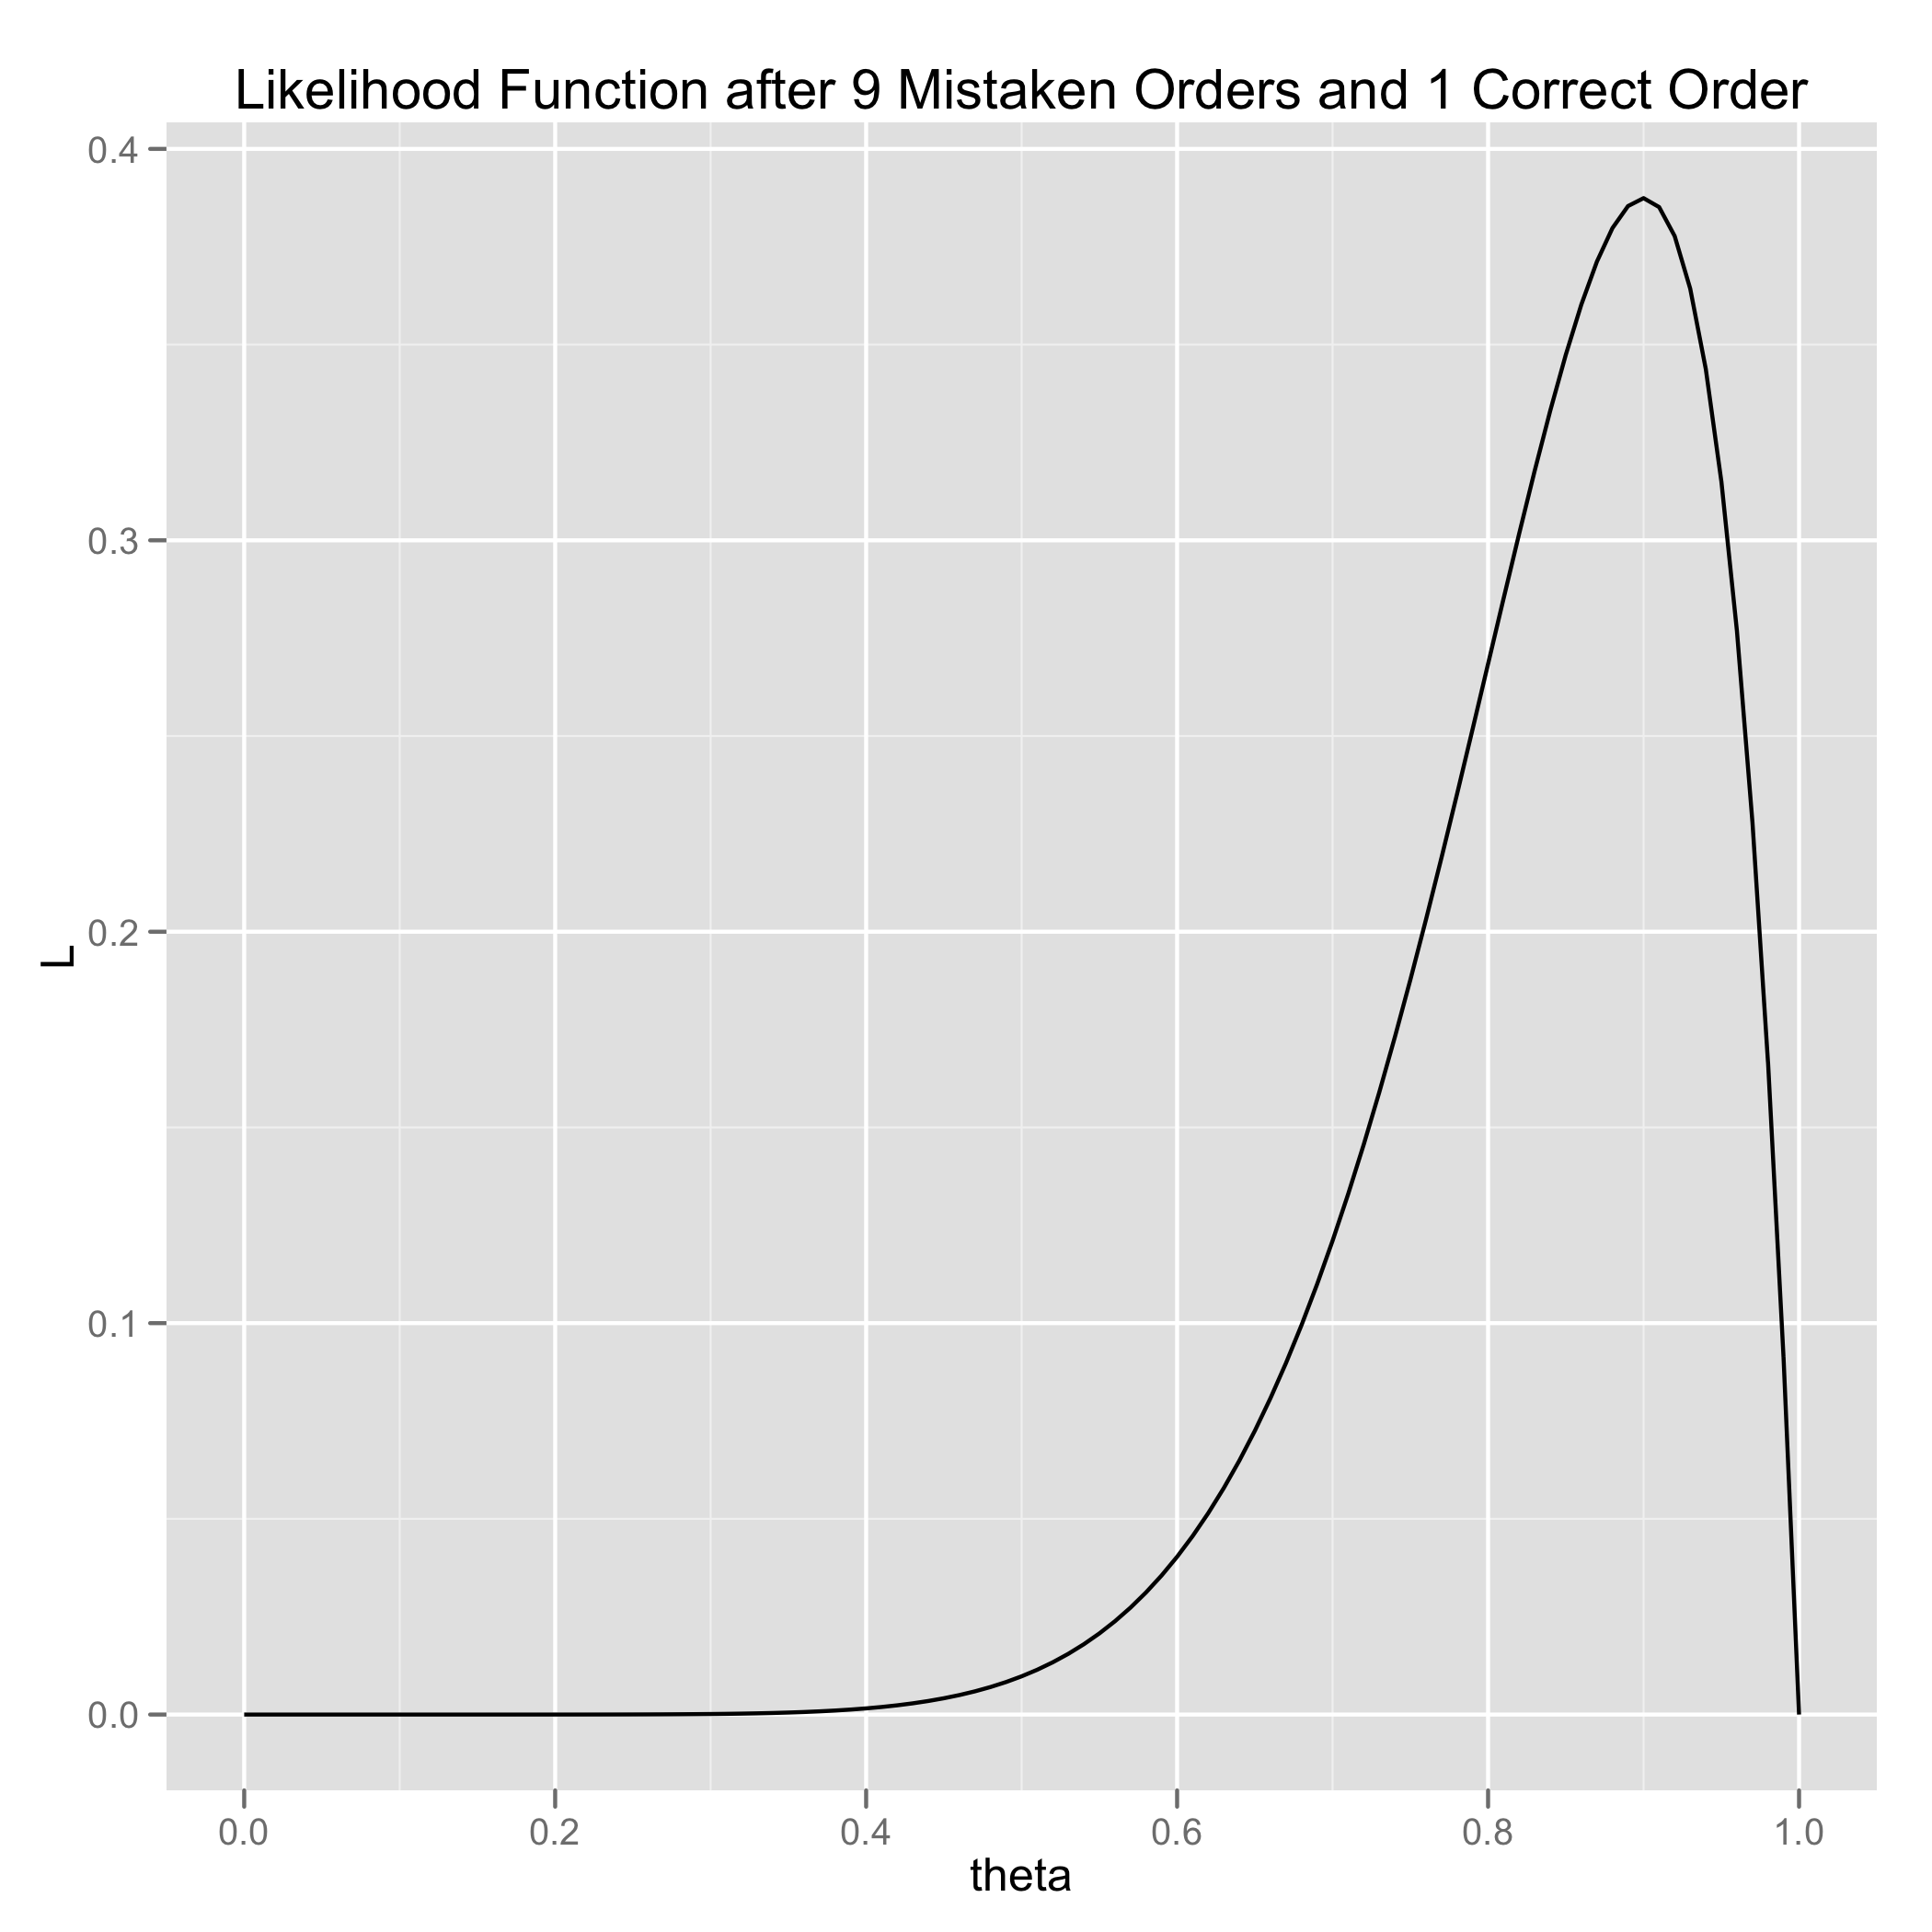
\includegraphics[scale = 0.1]{likelihood_function.png}
  \end{center}
}

\frame
{
  \begin{center}
    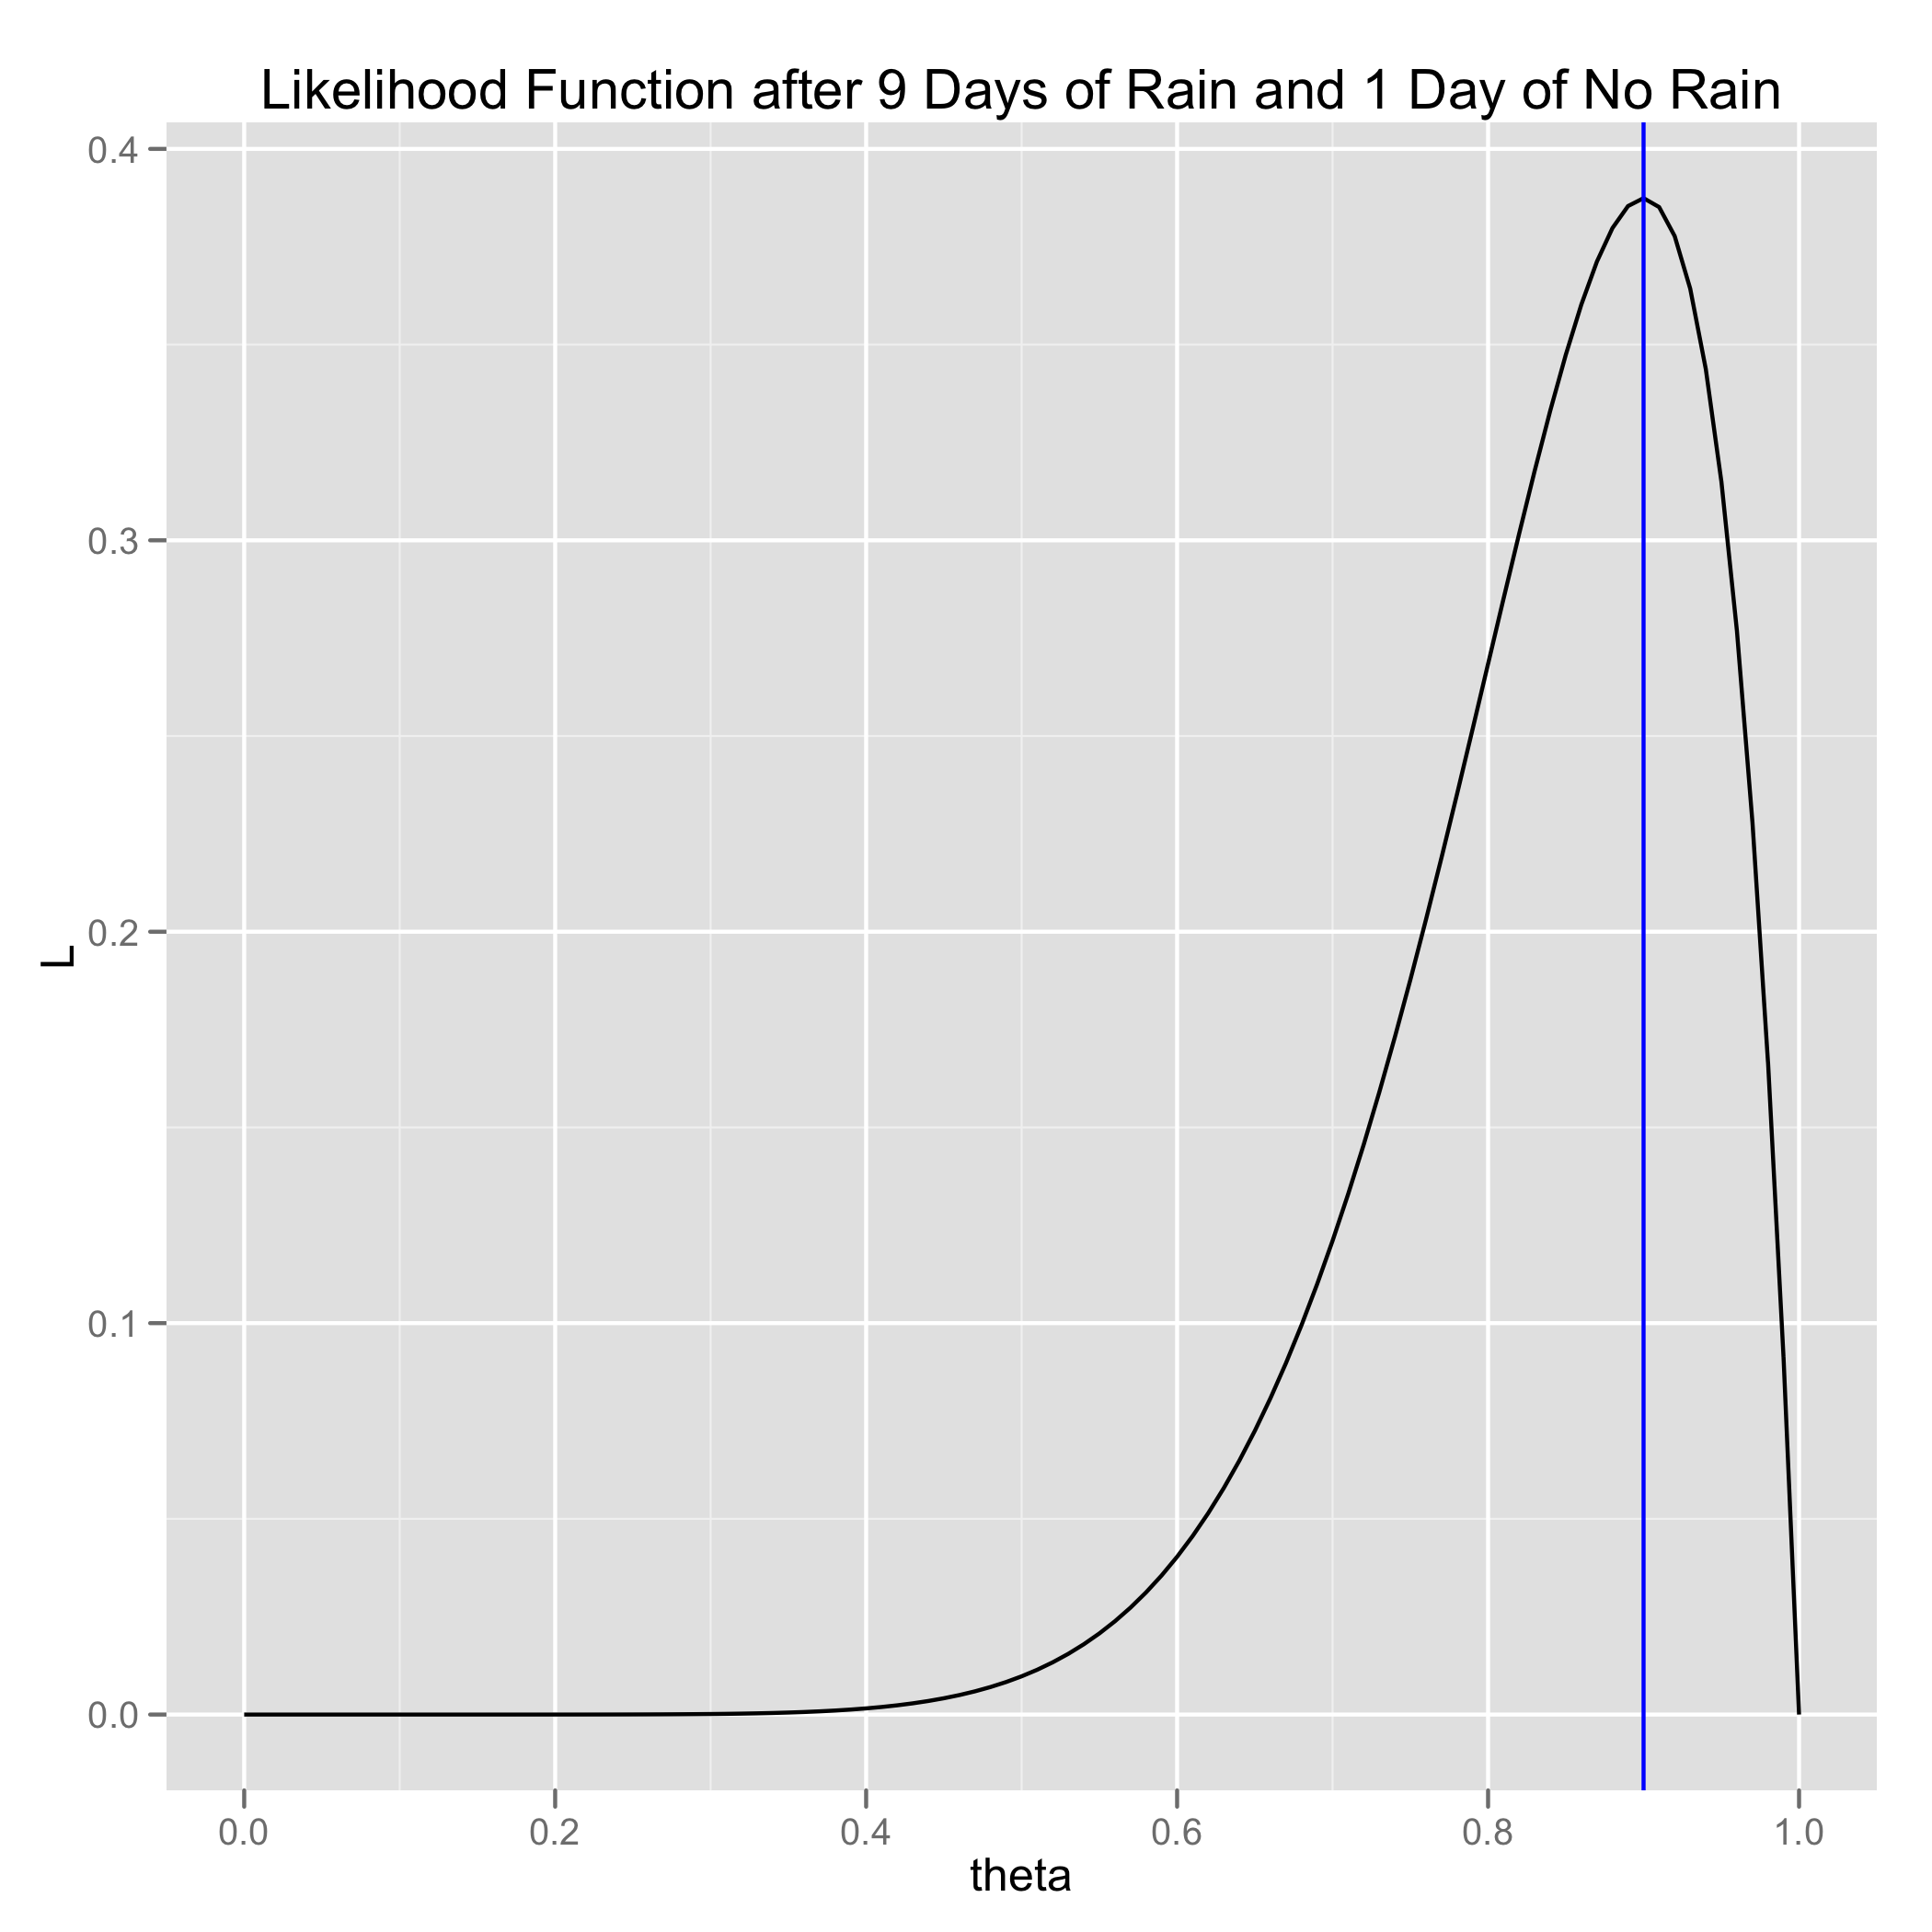
\includegraphics[scale = 0.1]{likelihood_function_mle.png}
  \end{center}
}

\frame
{
 \begin{itemize}
   \item{We've seen mistakes in 90\% of our orders}
   \item{The likelihood function has a single peak at $\theta = 0.9$}
   \item{We might guess that we can estimate $\theta$ by maximizing the likelihood function}
 \end{itemize}
}

\frame
{
  \begin{itemize}
    \item{Estimating parameters by maximizing the likelihood function is a good general strategy}
    \item{It also seems intuitively reasonable:}
    \begin{quote}
If we had to predict the future from our model, we should use parameter values that would increase our chances of predicting the data from the past
\end{quote}
  \end{itemize}
}

\frame
{
  \begin{itemize}
    \item{For our example model, maximizing the likelihood function can be done analytically}
    \item{In other models, computational methods are required}
  \end{itemize}
}

\frame
{
  \begin{itemize}
    \item{Note that the maximum of}
  \[
  \binom{n - 1}{n} \theta ^ {n - 1} (1 - \theta)
  \]
    \item{occurs at the same place as the maximum of}
  \[
  \theta ^ {n - 1} (1 - \theta)
  \]
  \end{itemize}
}

\frame
{
  \begin{itemize}
    \item{Then note that the maximum of}
  \[
  \theta ^ {n - 1} (1 - \theta)
  \]
    \item{occurs at the same place as the maximum of}
  \[
  \log[\theta ^ {n - 1} (1 - \theta)] = (n -1) \log[\theta] + \log[1 - \theta]
  \]
  \end{itemize}
}

\frame
{
  \begin{itemize}
    \item{The default parameter estimation strategy of maximizing the log likelihood function comes from Fisher}
    \item{Fisher demonstrated that it was a very powerful general strategy for estimating parameters}
  \end{itemize}
}

\frame
{
  \begin{itemize}
    \item{Prior to Fisher's work, statistics often involved the ad hoc construction of methods for estimating parameters}
    \item{Let's review those ideas, because they're important for thinking critically about Bayesian estimation}
  \end{itemize}
}

\frame
{
  \begin{itemize}
    \item{We'll call any function of our data a statistic}
    \item{Any statistic designed to give a point estimate of $\theta$ is an estimator}
  \end{itemize}
}

\frame
{
  \begin{itemize}
    \item{Suppose we have data that comes from a normal distribution with mean $\mu$}
    \item{How can we estimate $\mu$?}
  \end{itemize}
}

\frame
{
  \begin{itemize}
    \item{One estimator is the mean of the data}
    \item{Another is the median}
  \end{itemize}
}

\frame
{
  \begin{itemize}
    \item{How can we tell which of these two estimators works better?}
  \end{itemize}
}

\frame
{
  Sampling distribution analysis:
  \begin{itemize}
    \item{Suppose that $\theta$ is fixed}
    \item{We repeatedly sample random data sets from our model}
    \item{We compute our estimator on the resulting data sets}
    \item{We look at the distribution of our estimator after repeated sampling}
  \end{itemize}
}

\frame
{
  \begin{center}
    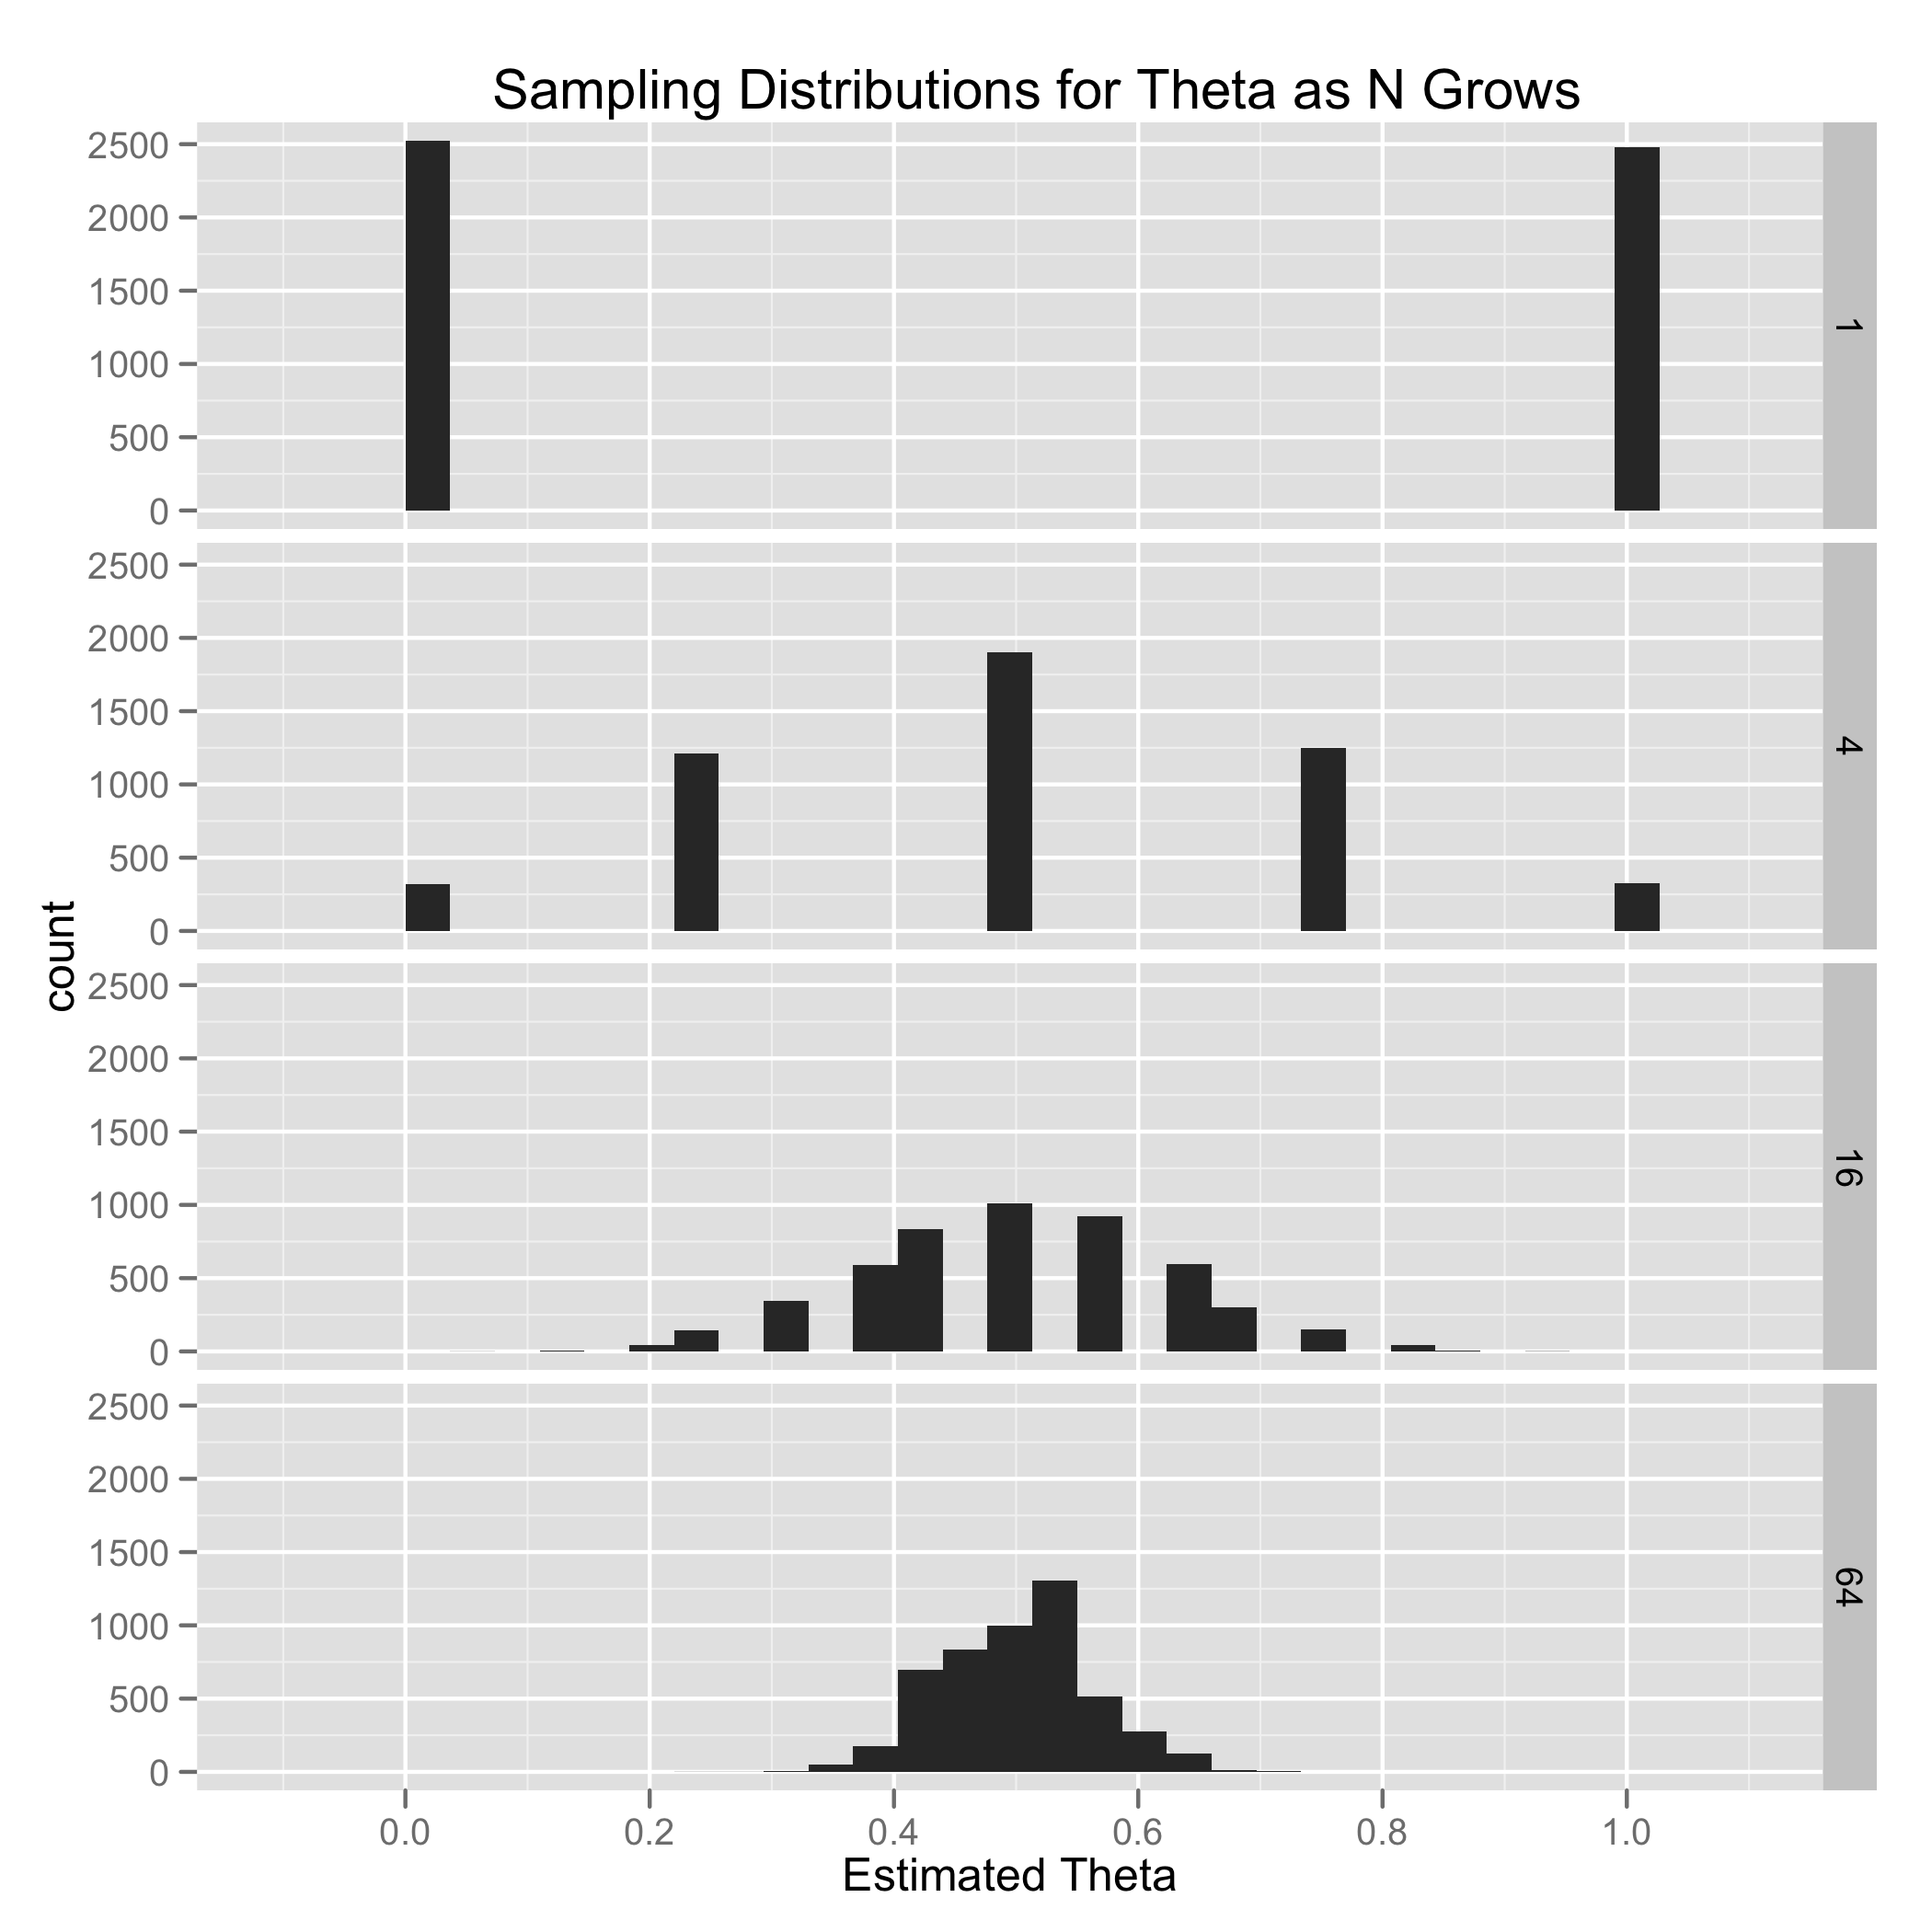
\includegraphics[scale = 0.1]{sampling_distribution.png}
  \end{center}
}

\frame
{
  \begin{itemize}
    \item{We then analyze the quality of an estimator by analyzing its sampling distribution}
  \end{itemize}
}

\frame
{
 Three criteria for selecting estimators are particularly popular:
 \begin{itemize}
   \item{Bias}
   \item{Variance}
   \item{Consistency}
 \end{itemize}
}

\frame
{
  \begin{itemize}
    \item{The bias of an estimator, $\hat{\theta}$, is}
    \[
    \mathbb{E}[\hat{\theta} - \theta] = \mathbb{E}[\hat{\theta}] - \theta
    \]
    \item{An unbiased estimator is one for which the mean of the sampling distribution is $\theta$}
    \item{In short, an unbiased estimator's expected value is $\theta$}
  \end{itemize}
}

\frame
{
  \begin{center}
    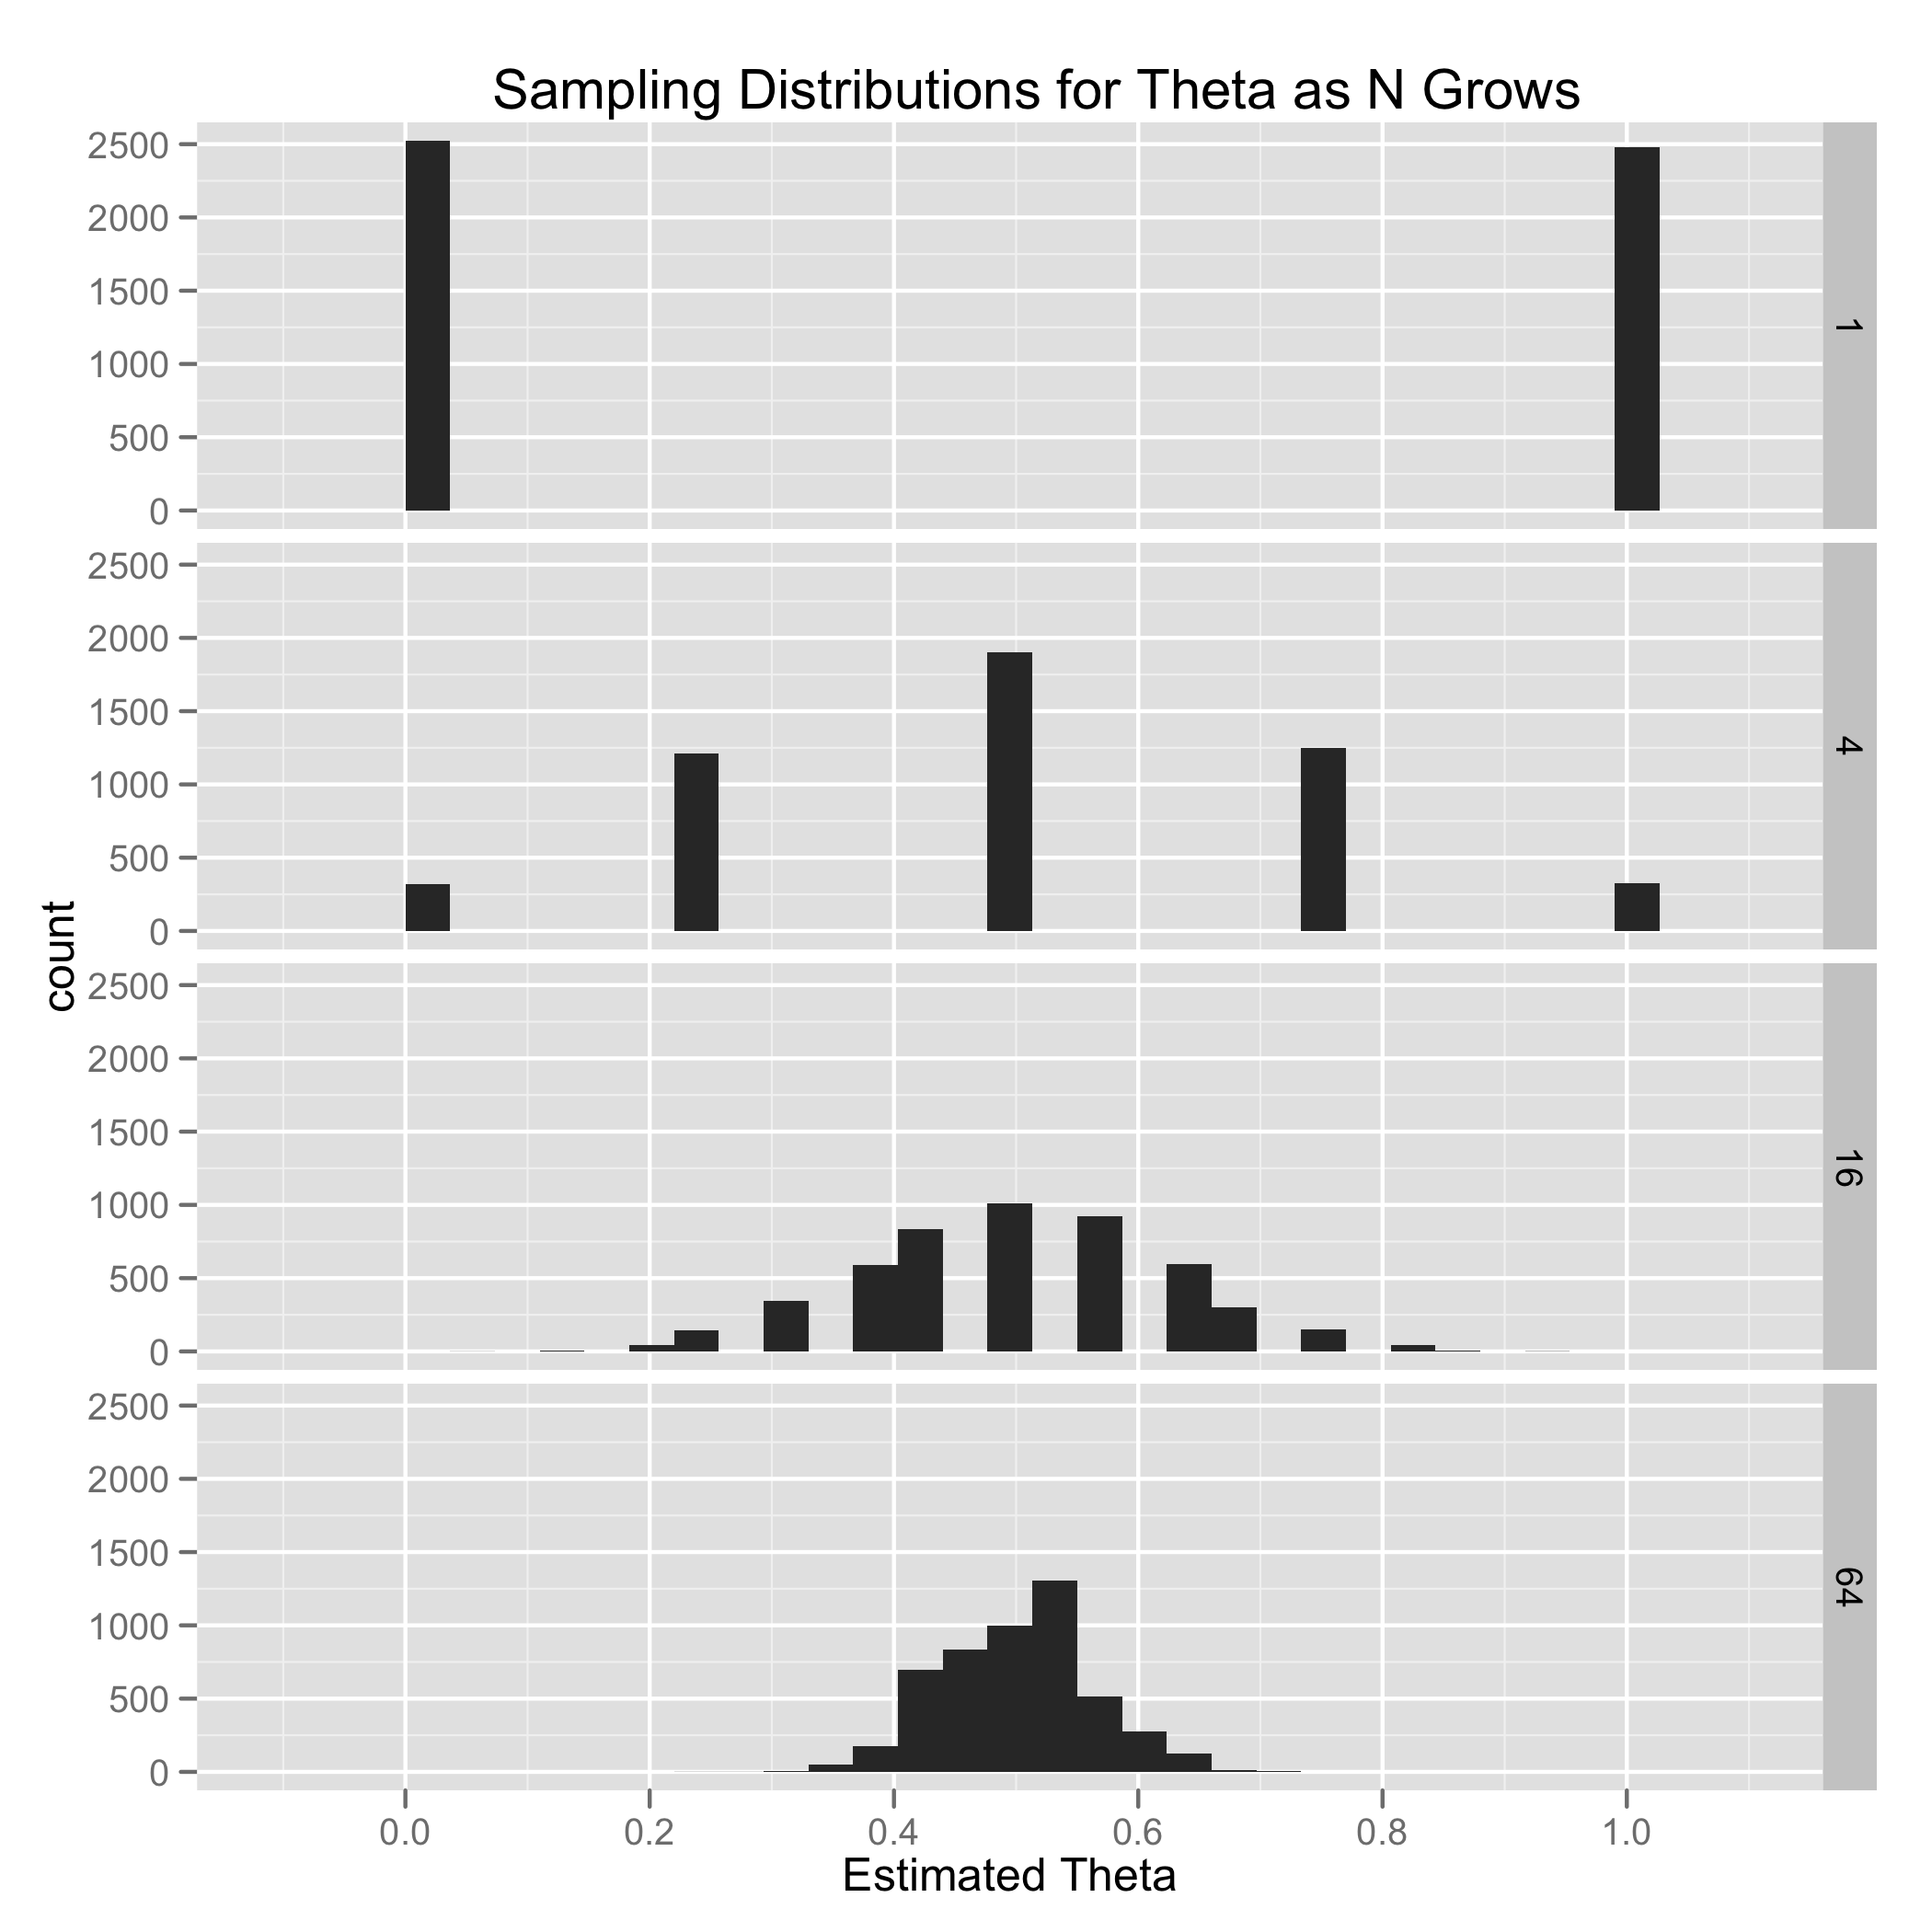
\includegraphics[scale = 0.1]{sampling_distribution.png}
  \end{center}
}

\frame
{
  \begin{itemize}
    \item{The variance of an estimator, $\hat{\theta}$, is}
    \[
    \mathbb{E}[(\hat{\theta} - \mathbb{E}[\hat{\theta}]) ^ 2]
    \]
   \item{If the estimator is unbiased, the variance is the expected Euclidean distance between $\hat{\theta}$ and $\theta$}
   \item{In short, a low variance estimator is one that is typically close to $\mathbb{E}[\theta$]}
  \end{itemize}
}

\frame
{
  \begin{center}
    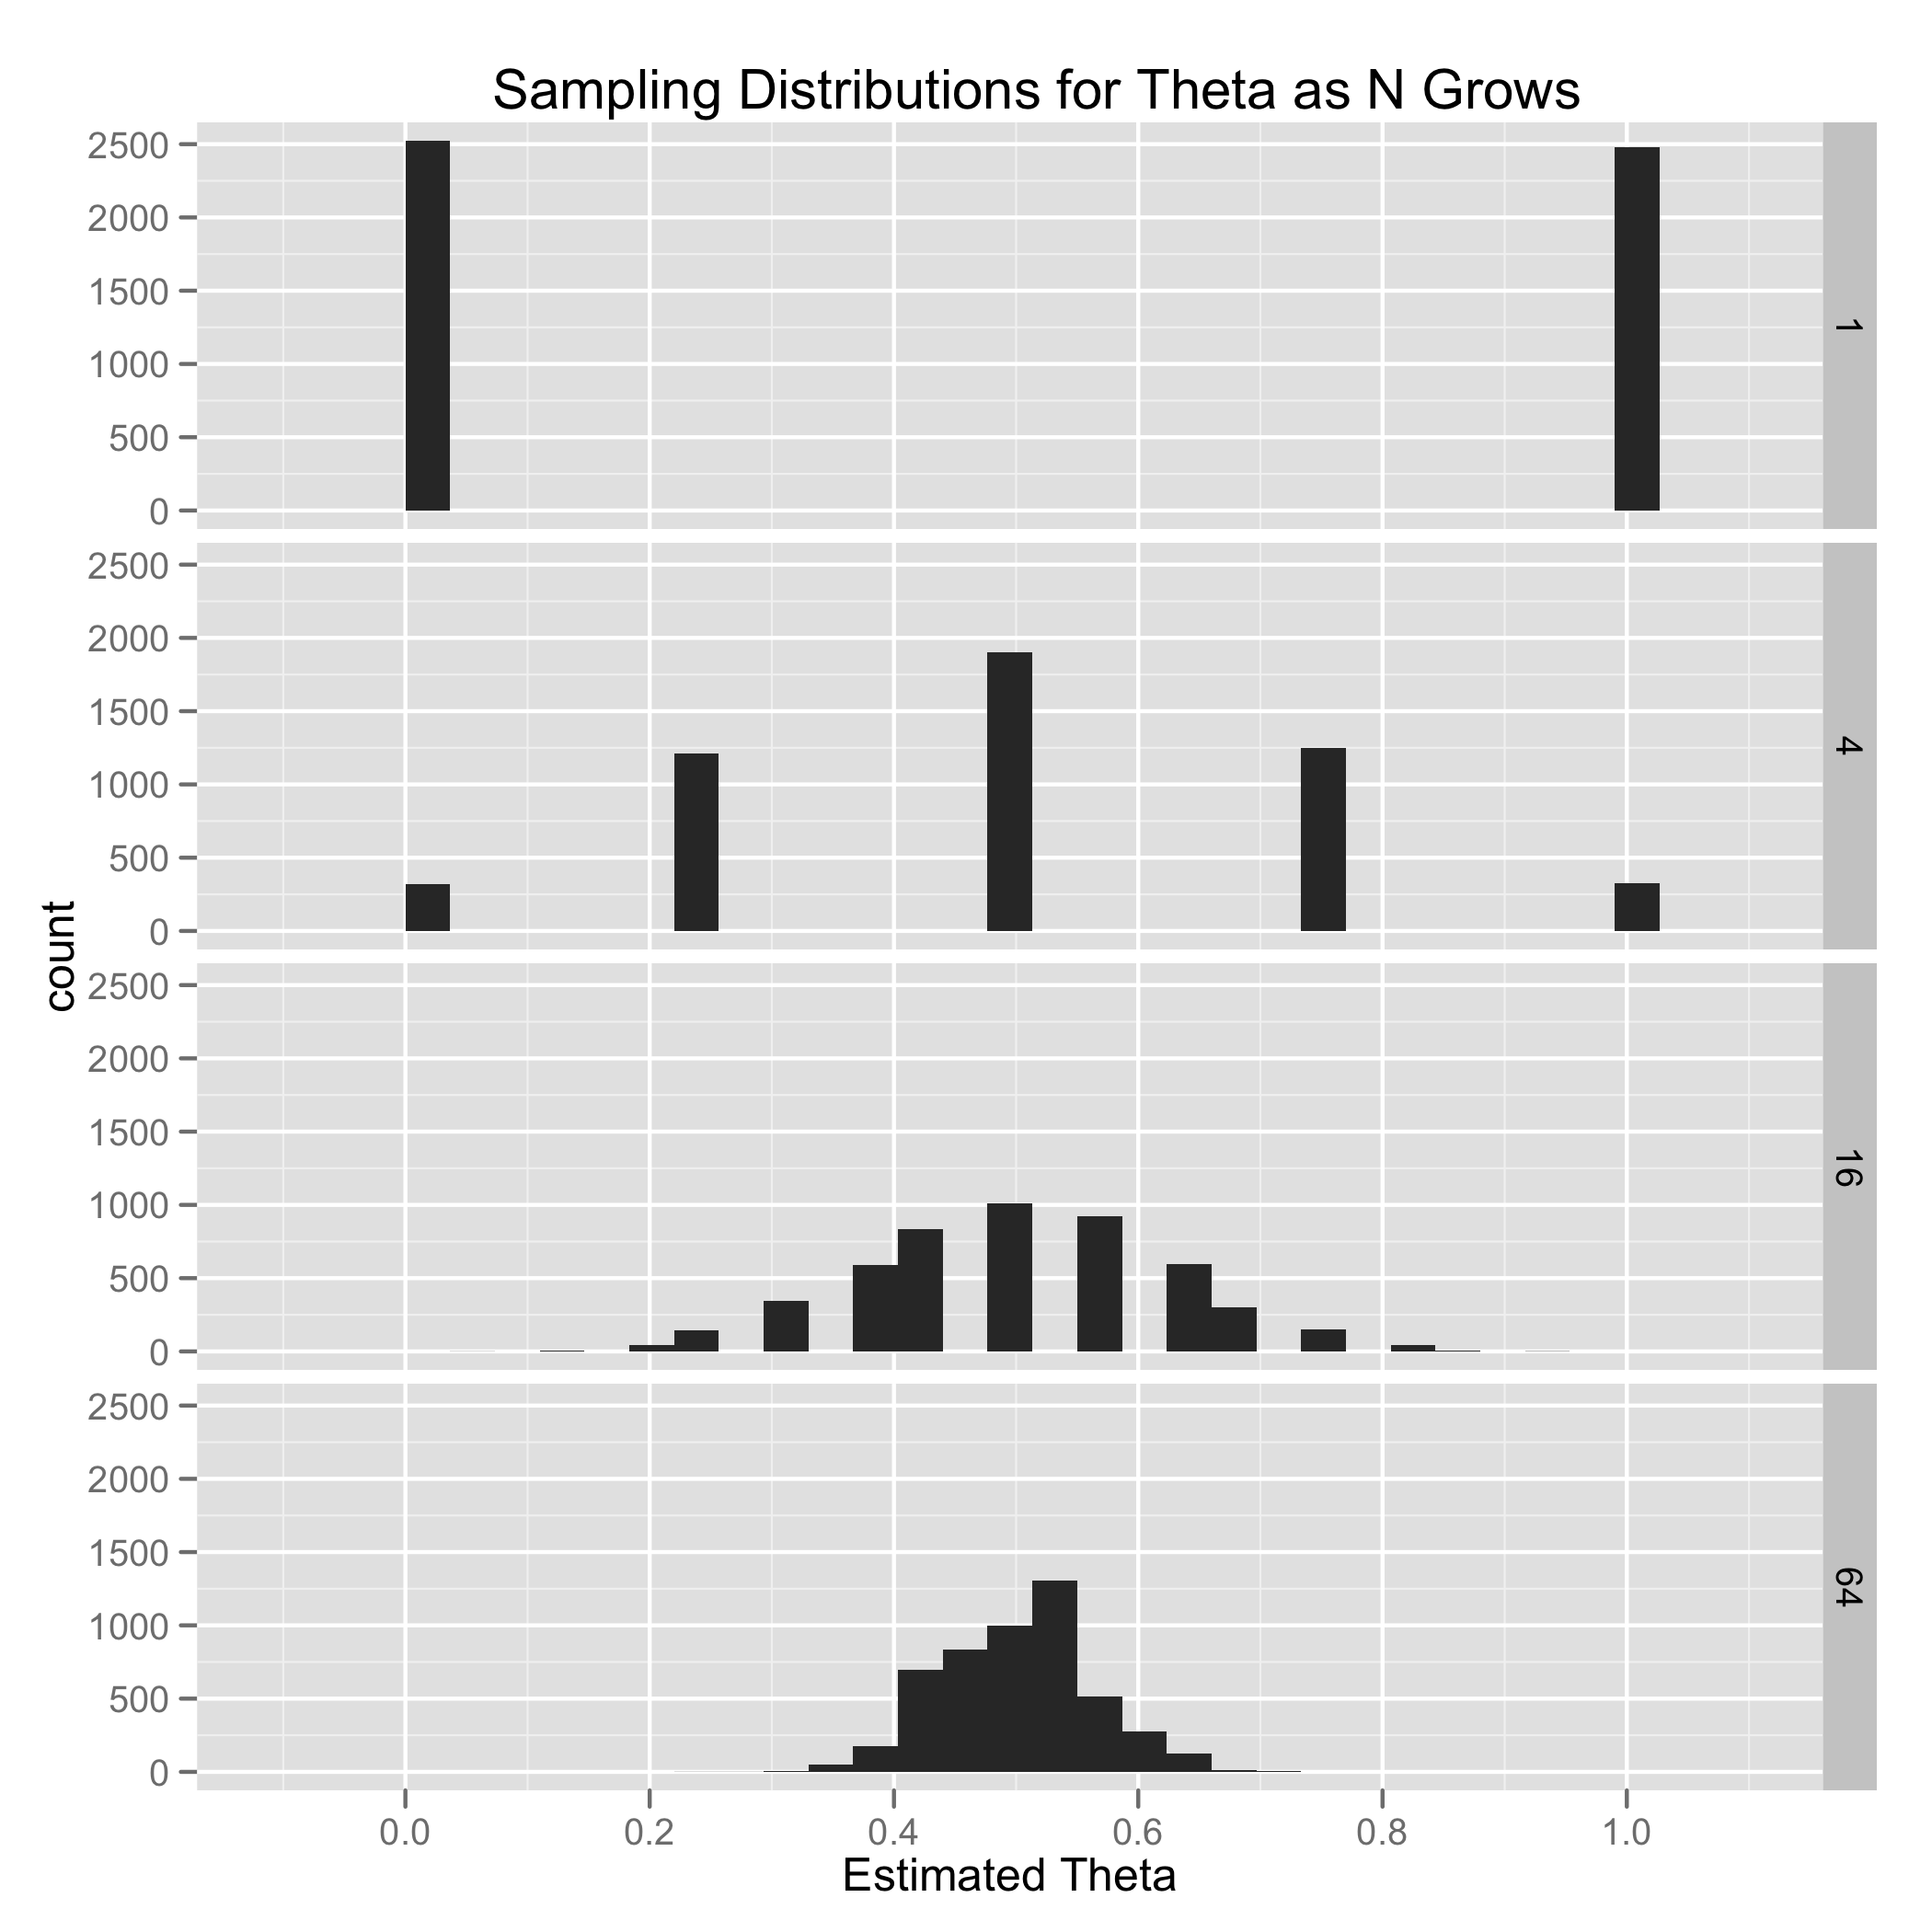
\includegraphics[scale = 0.1]{sampling_distribution.png}
  \end{center}
}

\frame
{
  \begin{itemize}
    \item{An estimator, $\hat{\theta}$, is consistent if}
    \[
    \lim_{n \to \infty} \hat{\theta} = \theta
    \]
    \item{A consistent estimator gets closer to $\theta$ as we get more data}
    \item{To be consistent, the bias and variance must both go to 0 as $n$ grows}
  \end{itemize}
}

\frame
{
  \begin{center}
    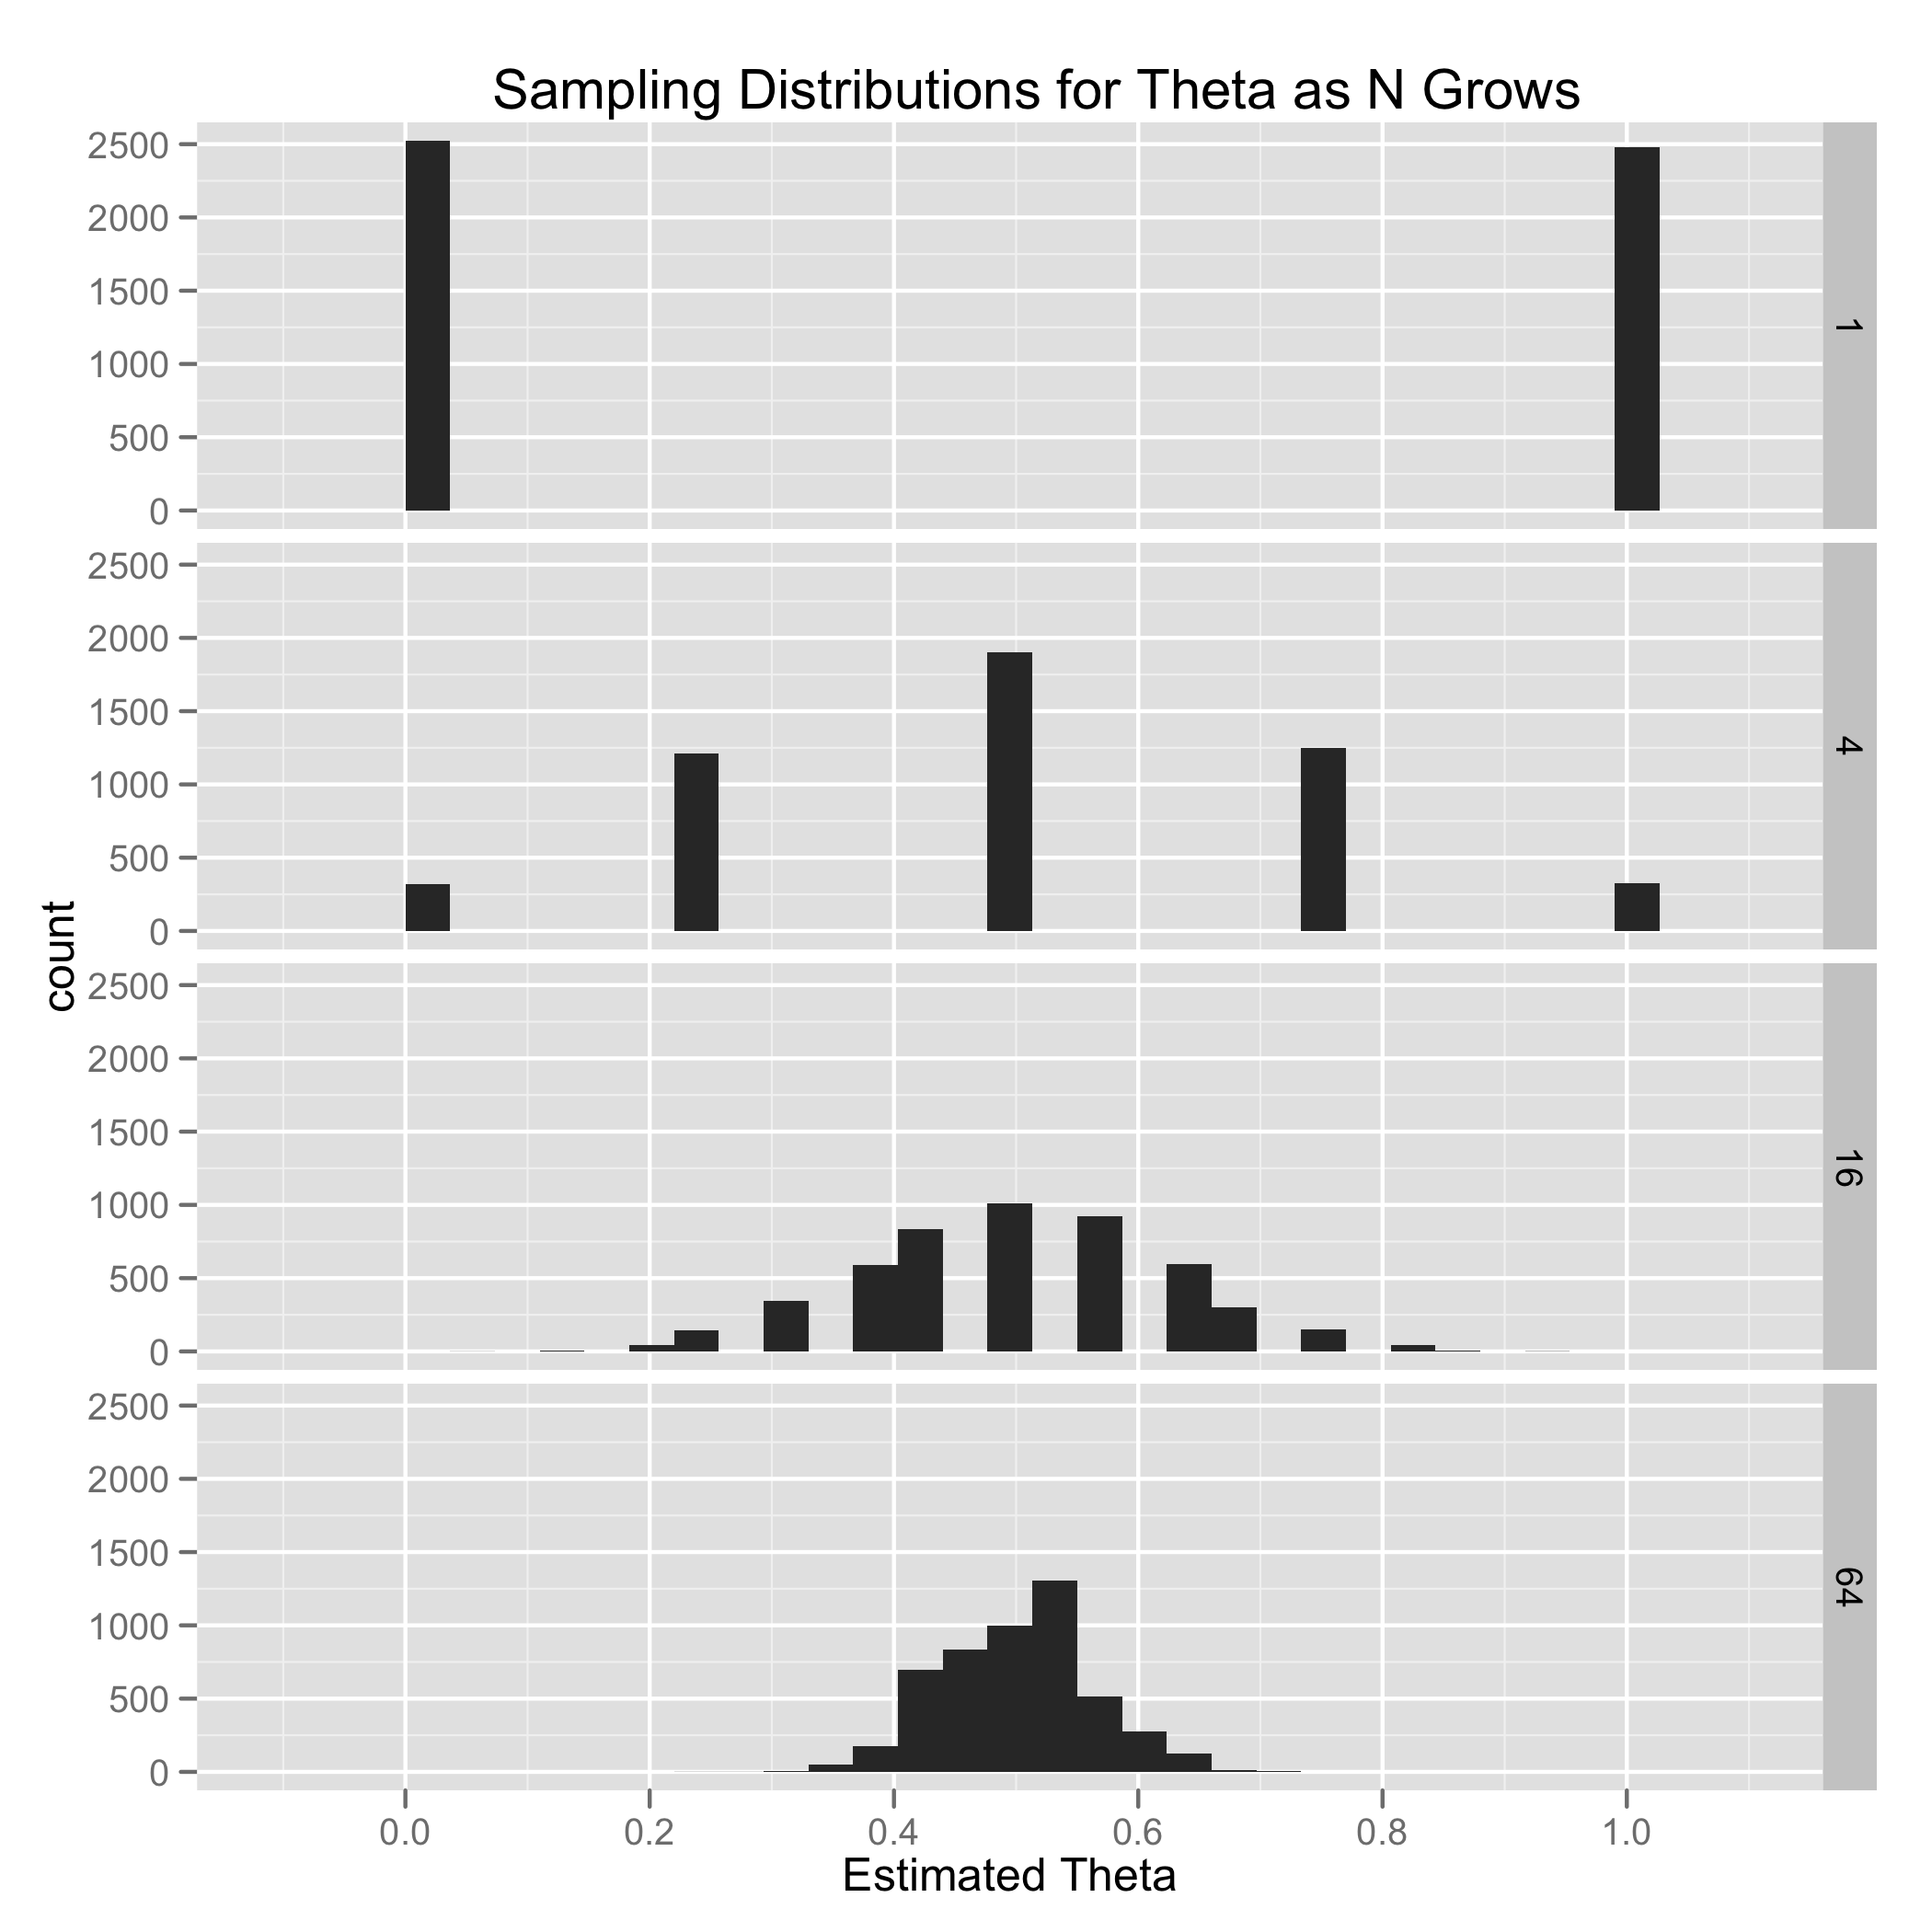
\includegraphics[scale = 0.1]{sampling_distribution.png}
  \end{center}
}

\frame
{
  \begin{itemize}
    \item{Fisher made the MLE popular by showing that typically:}
    \begin{itemize}
      \item{The MLE is unbiased}
      \item{The MLE is consistent}
      \item{The MLE is asymptotically the lowest variance estimator}
    \end{itemize}
  \end{itemize}
}

\frame
{
  \begin{itemize}
    \item{From the 1920's until the 1950's, the MLE was king}
    \item{In the 50's, James-Stein published a simple problem for which the MLE was a bad estimator}
  \end{itemize}
}

\frame
{
  \begin{itemize}
    \item{Since the 50's, interest has grown in alternative estimation strategies }
    \item{It is now clear that unbiased estimators are sometimes bad in practice}
    \item{It is now clear that finite sample behavior is not the same as asymptotic behavior}
  \end{itemize}
}

\frame
{
  \begin{itemize}
    \item{Enter the Bayesian estimation strategy}
    \item{In many practical problems, Bayesian methods are biased}
    \item{But, in many practical problems, Bayesian methods have lower variance than MLE methods}
    \item{Moreover, bias and variance can often be explicitly traded off}
  \end{itemize}
}

\frame
{
  \begin{itemize}
    \item{Let's go back to the likelihood function}
    \item{We've seen one way of using it to construct estimators}
    \item{What other information can we get from it?}
  \end{itemize}
}

\frame
{
  \begin{itemize}
    \item{We can get a measure of our uncertainty about $\theta$}
    \item{We do this by looking at the curvature of the likelihood function}
    \item{Formally, this is the Fisher information}
  \end{itemize}
}

\frame
{
  \begin{center}
    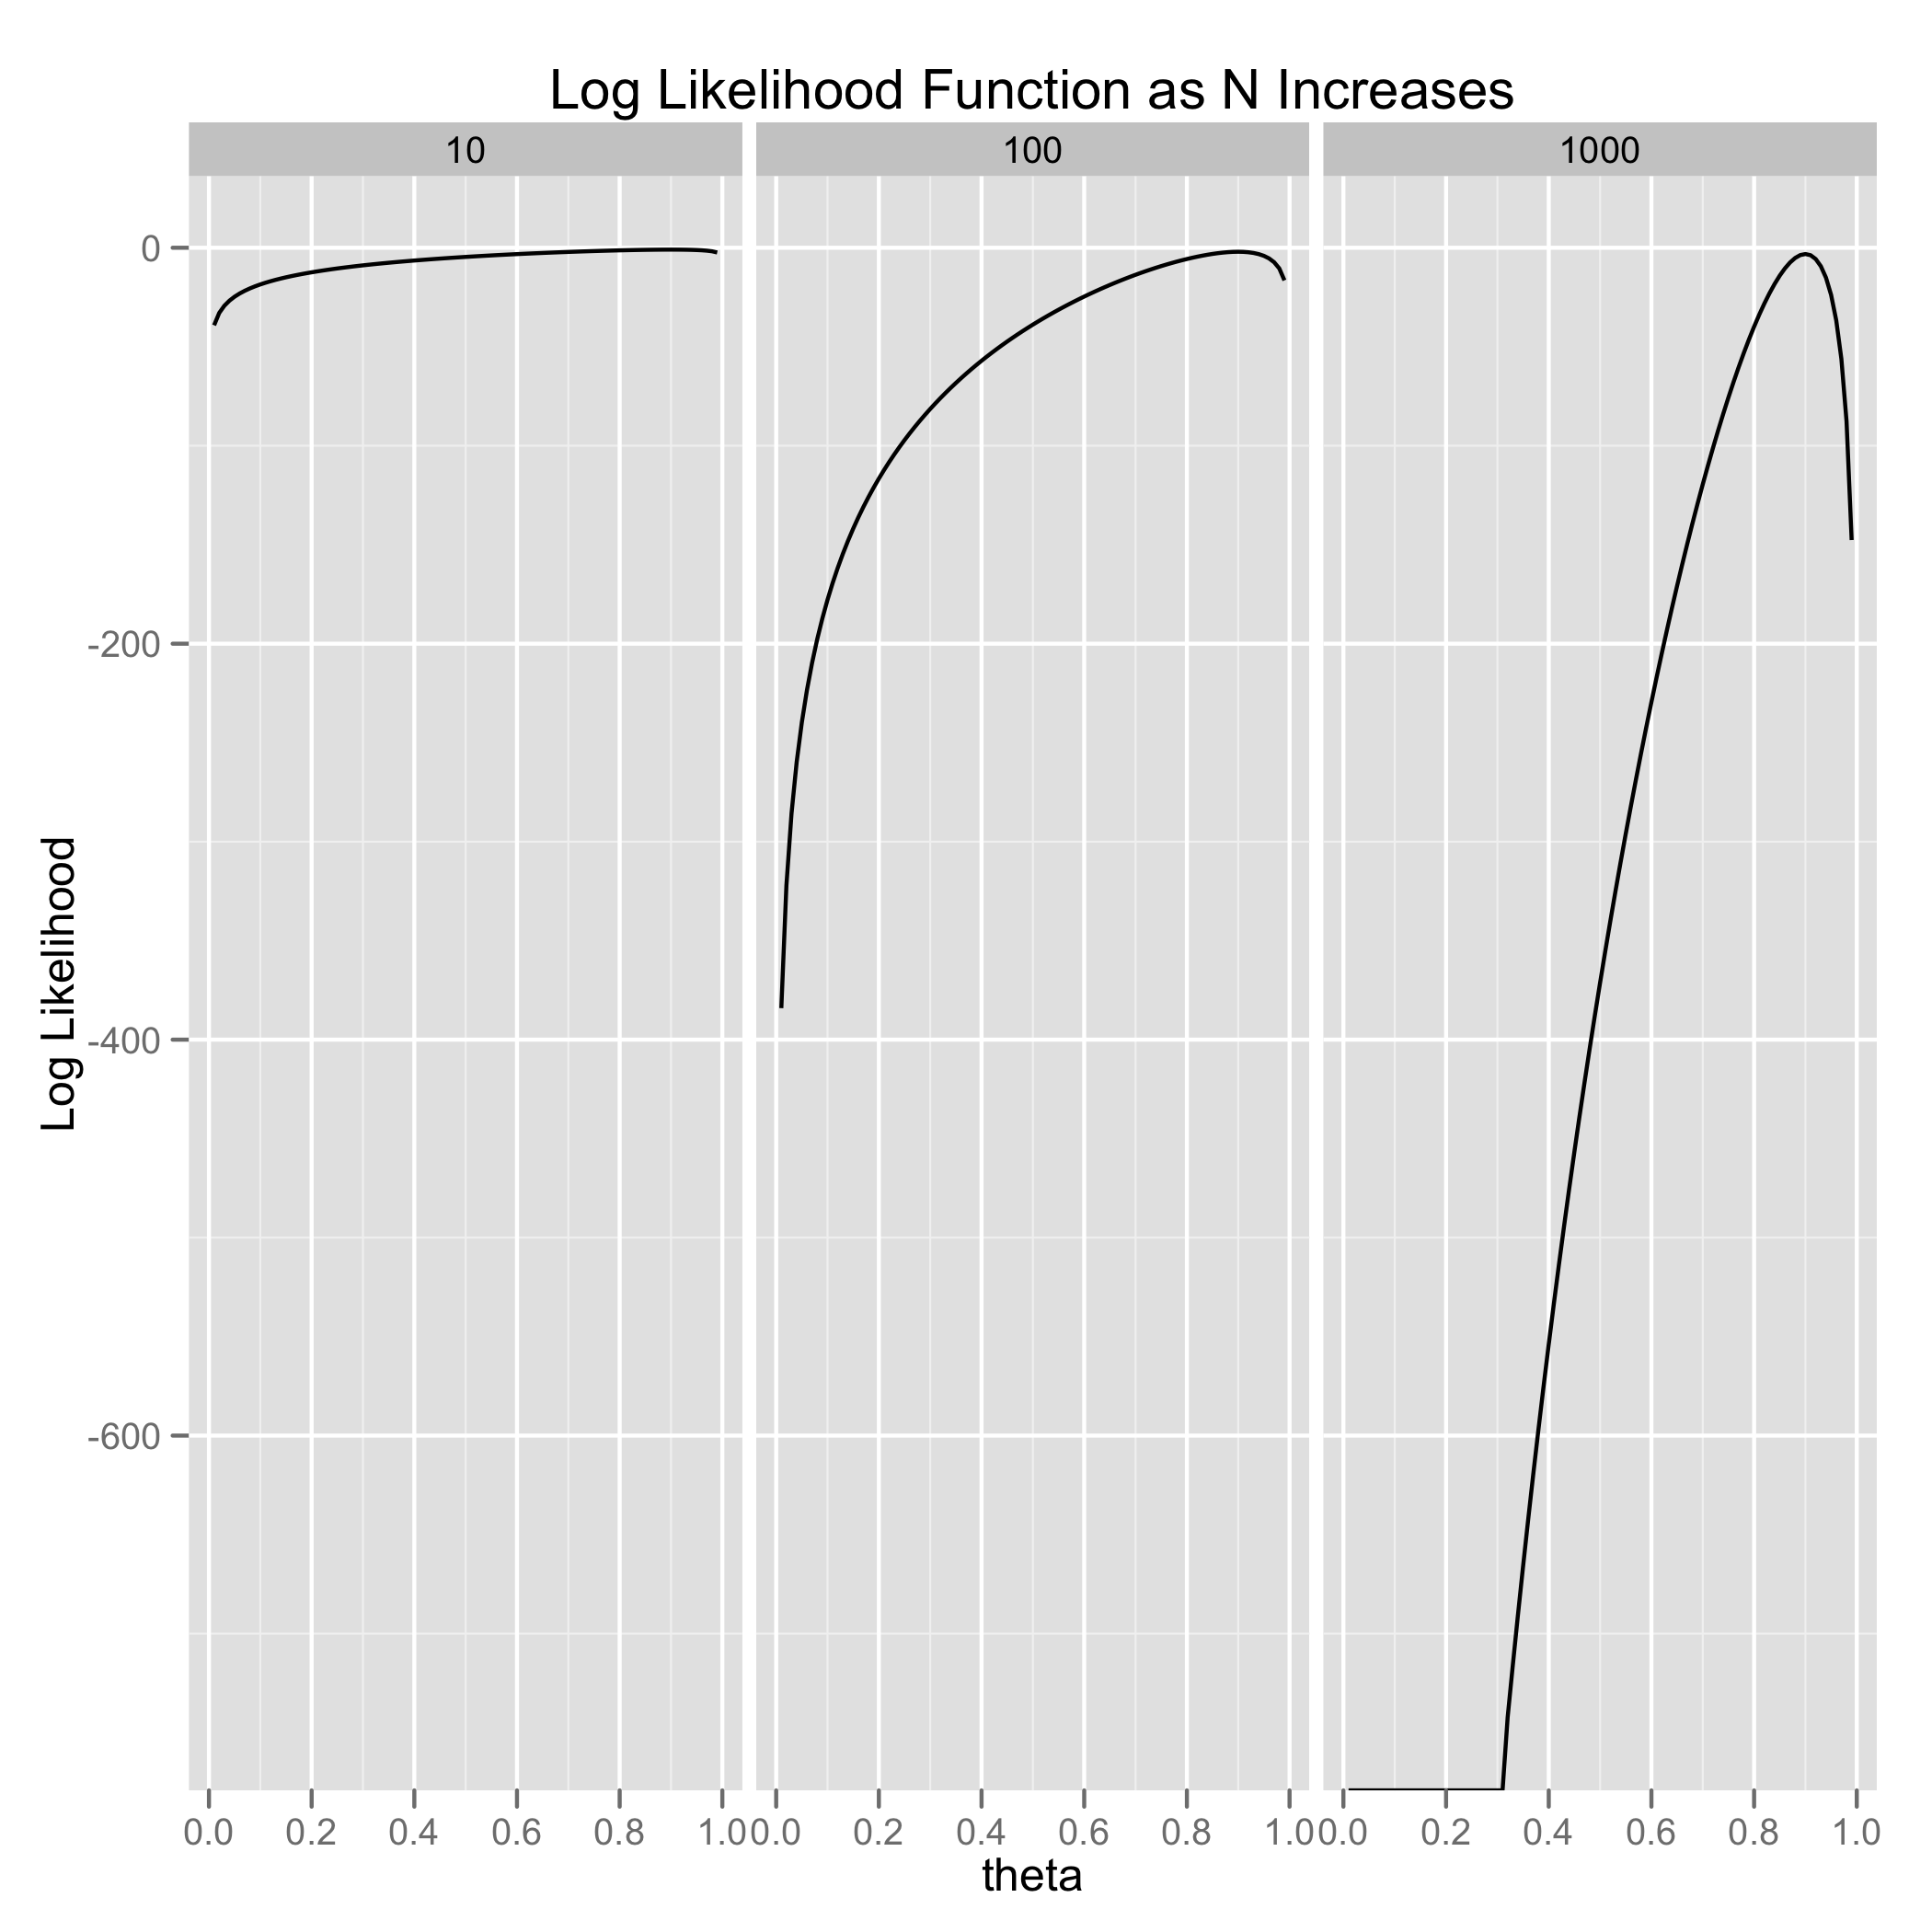
\includegraphics[scale = 0.1]{fisher_information.png}
  \end{center}
}

\frame
{
  \begin{itemize}
    \item{We've now seen that we can learn a lot from the likelihood function}
    \begin{itemize}
      \item{The peak gives us an estimator}
      \item{The spread gives us a sense of uncertainty}
    \end{itemize}
  \end{itemize}
}

\frame
{
  \begin{itemize}
    \item{Pushing on these ideas, we might wish to have a single numeric language for representing our knowledge of $\theta$ that organizes the information in the likelihood function}
    \item{For a Bayesian that language is probability theory}
    \item{We'd like to say that we think that $\hat{\theta}$ is the most probable value for $\theta$}
    \item{We'd also like to say that there is a 95\% chance that $\theta$'s value is in some interval, $[a, b]$}
  \end{itemize}
}

\frame
{
  \begin{itemize}
    \item{We start with a probability distribution over $\theta$: $p(\theta)$}
    \item{We call this distribution our prior}
    \item{It is a prior because it represents our beliefs before we see data}
  \end{itemize}
}

\frame
{
  \begin{itemize}
    \item{We wish to calculate our belief distribution after seeing data, $D$:
$p(\theta | D)$}
    \item{We call this distribution our posterior}
    \item{It is a posterior because it represents our beliefs after we see data}
  \end{itemize}
}

\frame
{
  \begin{itemize}
    \item{We can calculate our posterior using Bayes' theorem:}
\[
p(\theta | x_1, \ldots, x_n) = \frac{p(x_1, \ldots, x_n | \theta) p(\theta)}{p(x_1, \ldots, x_n)}
\]
  \end{itemize}
}

\frame
{
  \begin{itemize}
    \item{$p(D)$ is called the evidence. It is a constant}
    \item{Therefore}
    \[
    p(\theta | D) \propto p(D | \theta) p(\theta)
    \]
  \end{itemize}
}

\frame
{
 In words:
 \begin{itemize}
   \item{Up to a scaling factor, the value of our posterior at a point $\theta^{*}$ is the product of the likelihood function evaluated at $\theta^{*}$ and the prior evaluated at $\theta^{*}$}
   \item{If our prior is flat, the posterior's shape is the likelihood function's shape}
 \end{itemize}
}

\frame
{
  \begin{itemize}
    \item{In practice calculating the posterior is hard because the evidence can be impossible to calculate analytically}
    \item{But we can usually make good approximations}
    \item{In some special circumstances, we can get analytic solutions}
  \end{itemize}
}

\frame
{
 Approximation strategy 1:
  \begin{itemize}
    \item{We want the posterior only at $n$ points on a grid}
    \item{We find the unnormalized posterior by multiplying the likelihood and prior}
    \item{We evaluate the approximate evidence by summing the unnormalized posterior}
    \item{We divide the unnormalized posterior by the approximate evidence to get a proper probability distribution}
  \end{itemize}
}

\frame
{
  \begin{itemize}
    \item{Suppose we start with a prior biased towards low values of $\theta$}
    \item{Then we see data for which the likelihood function supports high values of $\theta$}
    \item{The posterior describes our reconciliation of these two pieces of information}
  \end{itemize}
}

\frame
{
  \begin{center}
    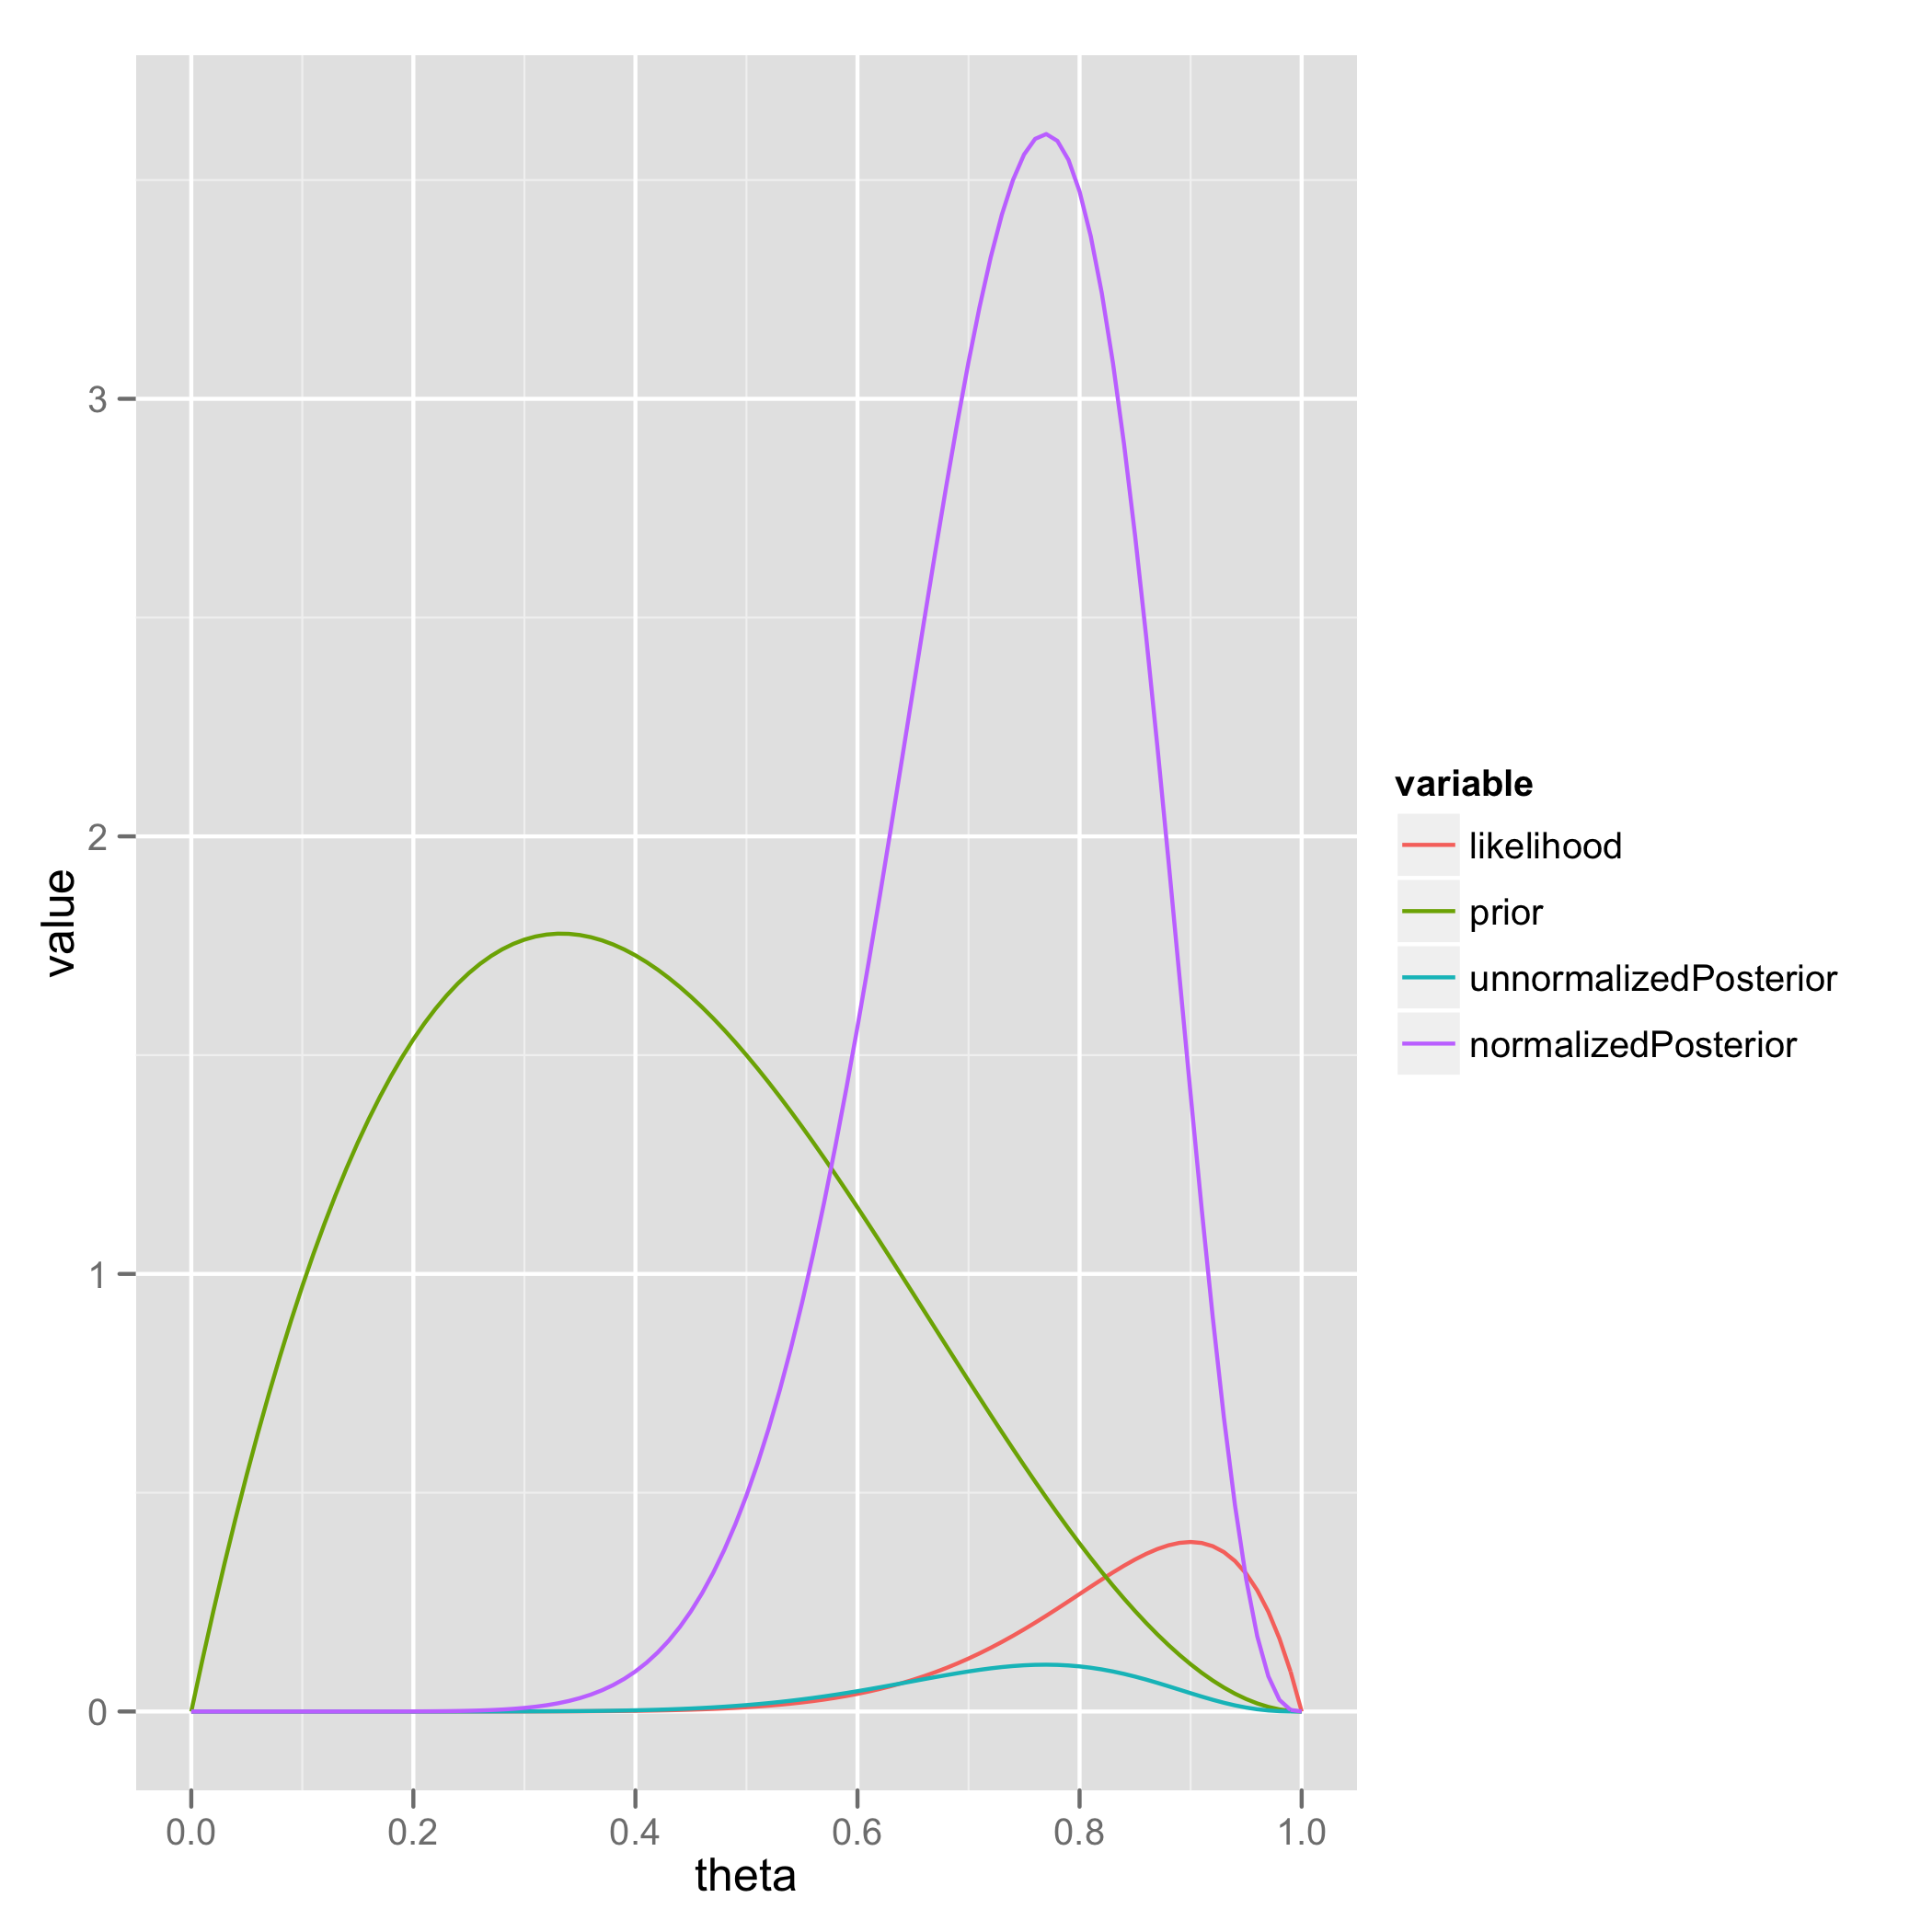
\includegraphics[scale = 0.1]{grid_approximation.png}
  \end{center}
}

\frame
{
  \begin{center}
    In this example, we can calculate the exact posterior for comparison
  \end{center}
}

\frame
{
  \begin{center}
    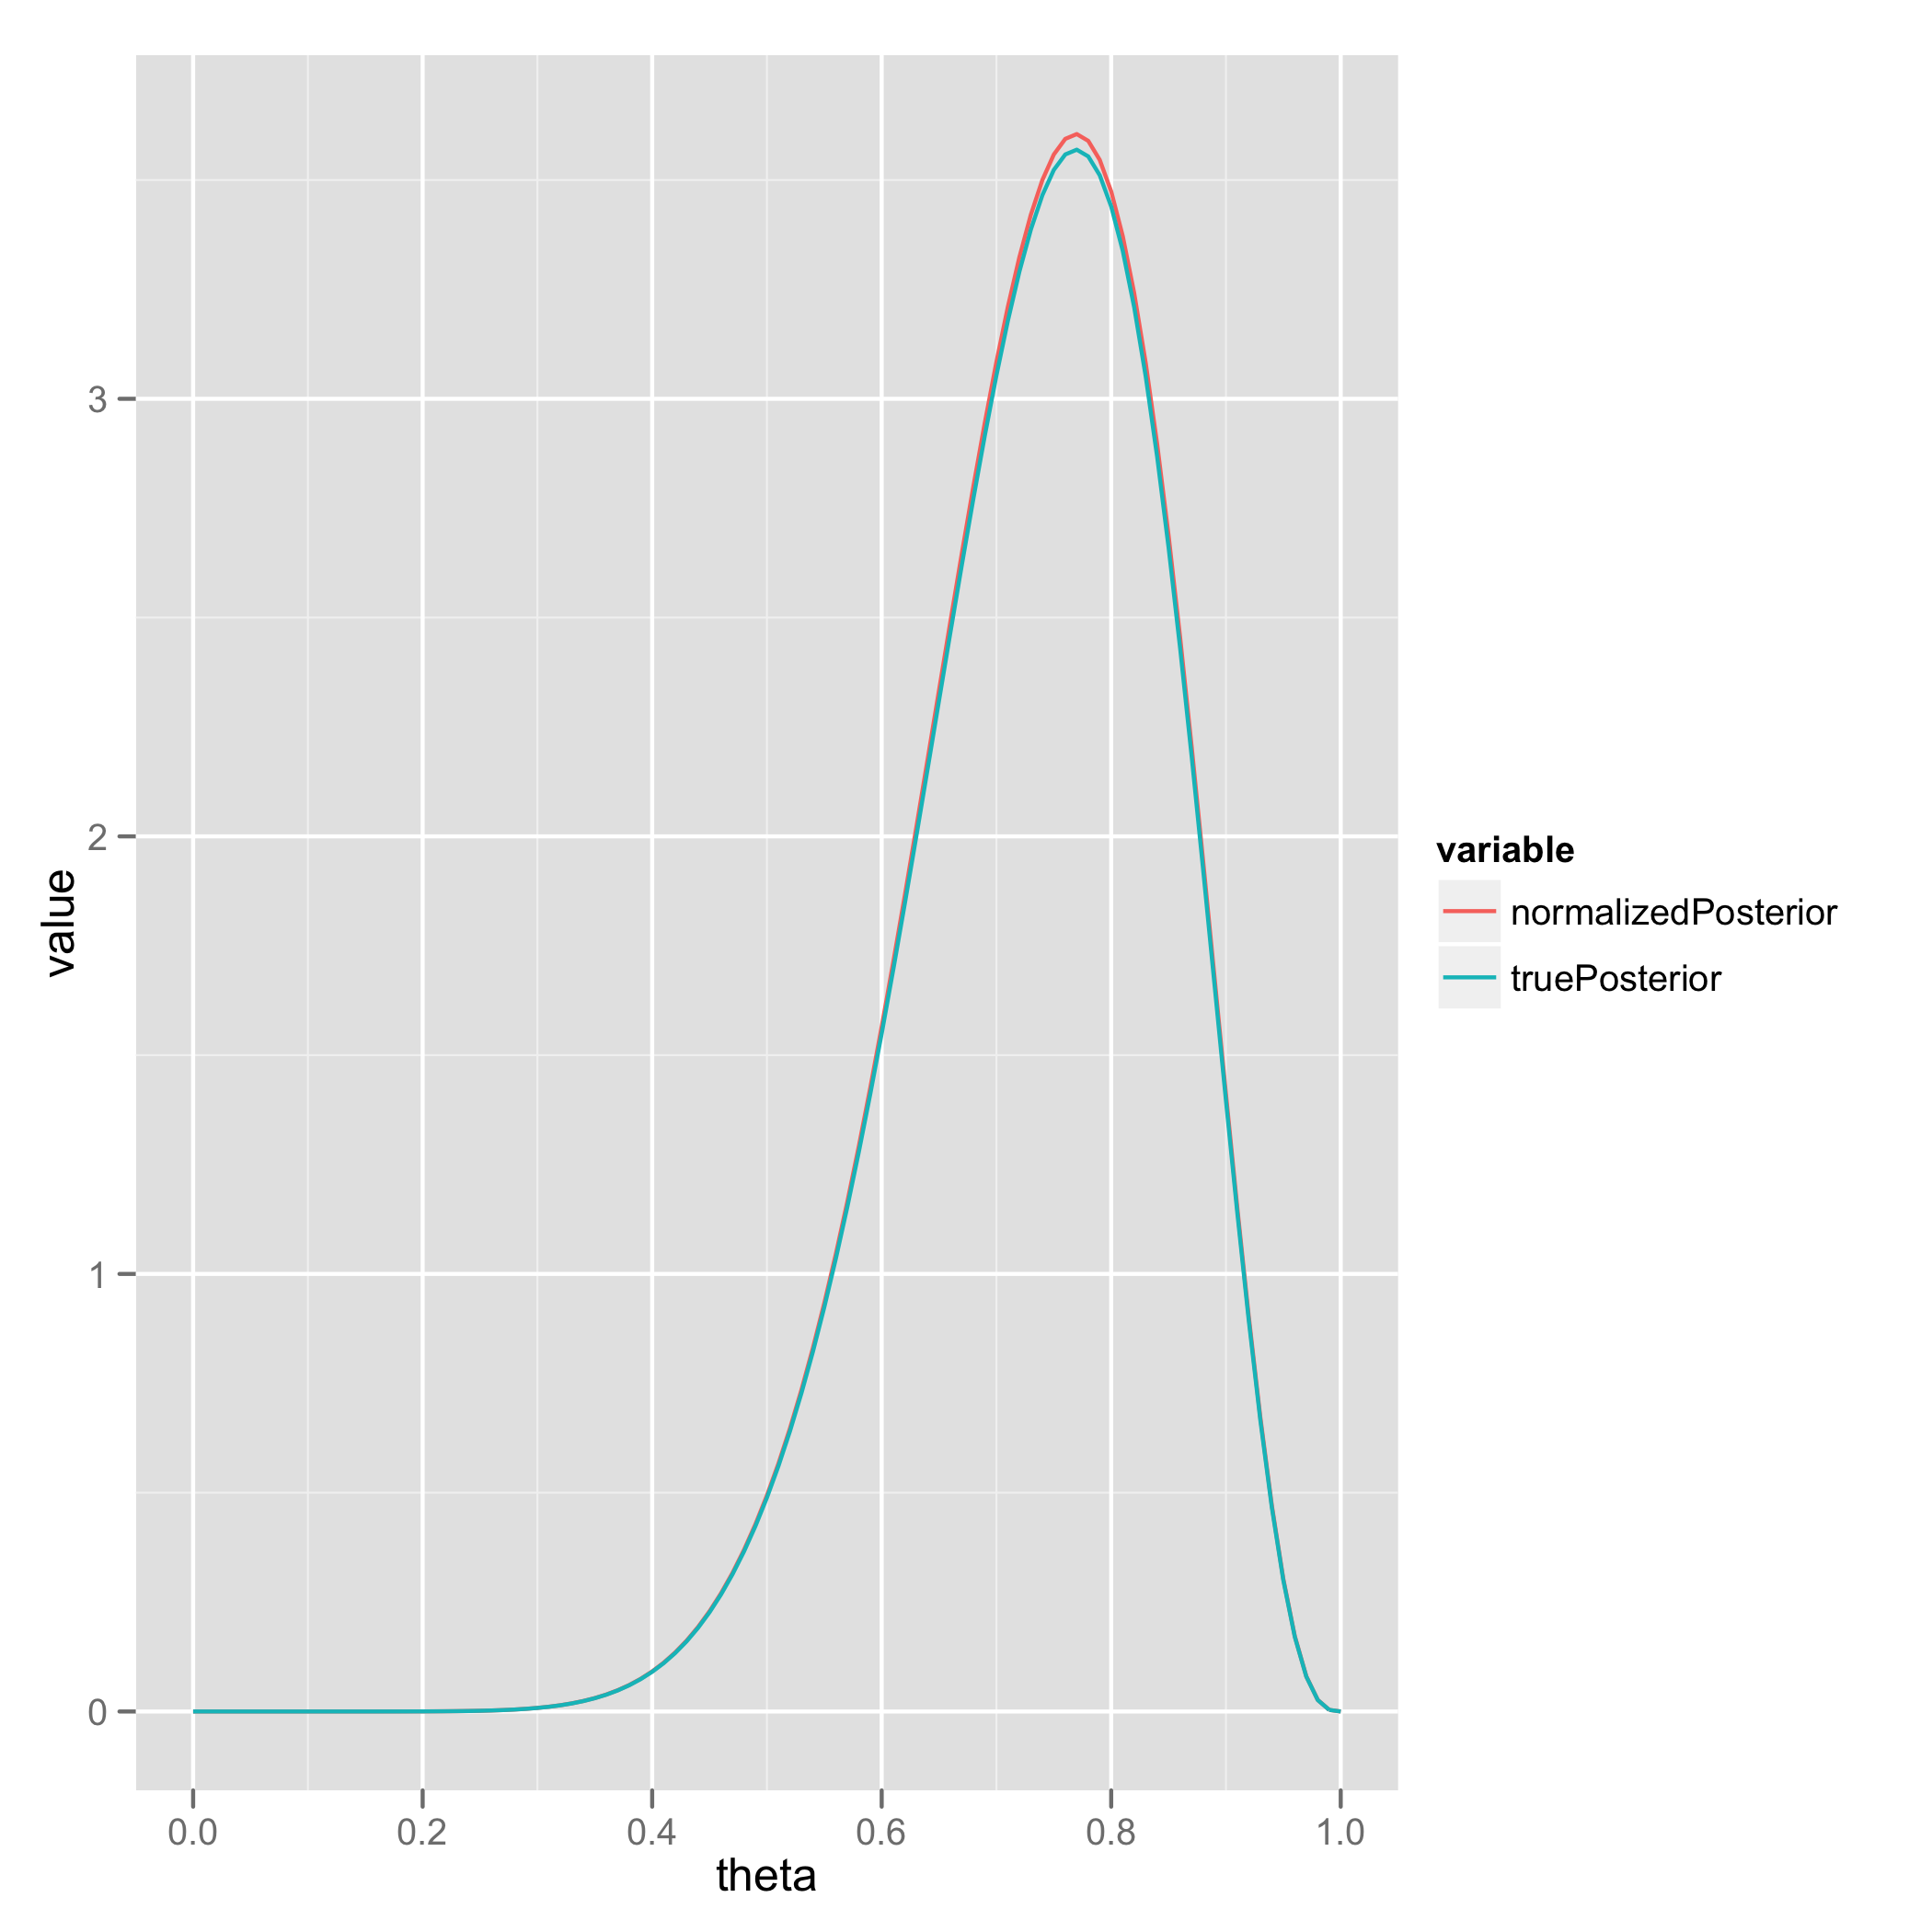
\includegraphics[scale = 0.1]{grid_quality.png}
  \end{center}
}

\frame
{
  \begin{itemize}
    \item{Here grid approximation works perfectly}
    \item{So where does grid approximation go wrong?}
    \item{Computational time and space is exponential in number of parameters in $\theta$}
    \item{Unclear how fine resolution of grid must be}
  \end{itemize}
}

\frame
{
  \begin{itemize}
    \item{There are important cases where analytic techniques work}
    \item{Given an appropriate prior, the posterior can have a closed form solution}
    \item{If both the prior and posterior have a constant functional form F, the prior is called conjugate}
  \end{itemize}
}

\frame
{
  \begin{itemize}
    \item{In our binomial example, a prior called the beta prior is conjugate to the binomial likelihood function}
    \item{The beta prior, $B(\alpha, \beta)$ has two parameters, $\alpha$ and $\beta$}
    \item{$\alpha$ is the number of 1's previously seen}
    \item{$\beta$ is the number of 0's previously seen}
    \item{After $x$ more 1's and $y$ more 0's, the posterior has the form}
    \[
      B(\alpha + x, \beta + y)
    \]
  \end{itemize}
}

\frame
{
  \begin{itemize}
    \item{Let's work further with our example}
    \item{Our prior will be a $B(2, 3)$ distribution}
    \item{We'll suppose we've seen 9 more mistaken orders and 1 correct order}
    \item{Our posterior is then a $B(11, 4)$ distribution}
  \end{itemize}
}

\frame
{
  \begin{center}
    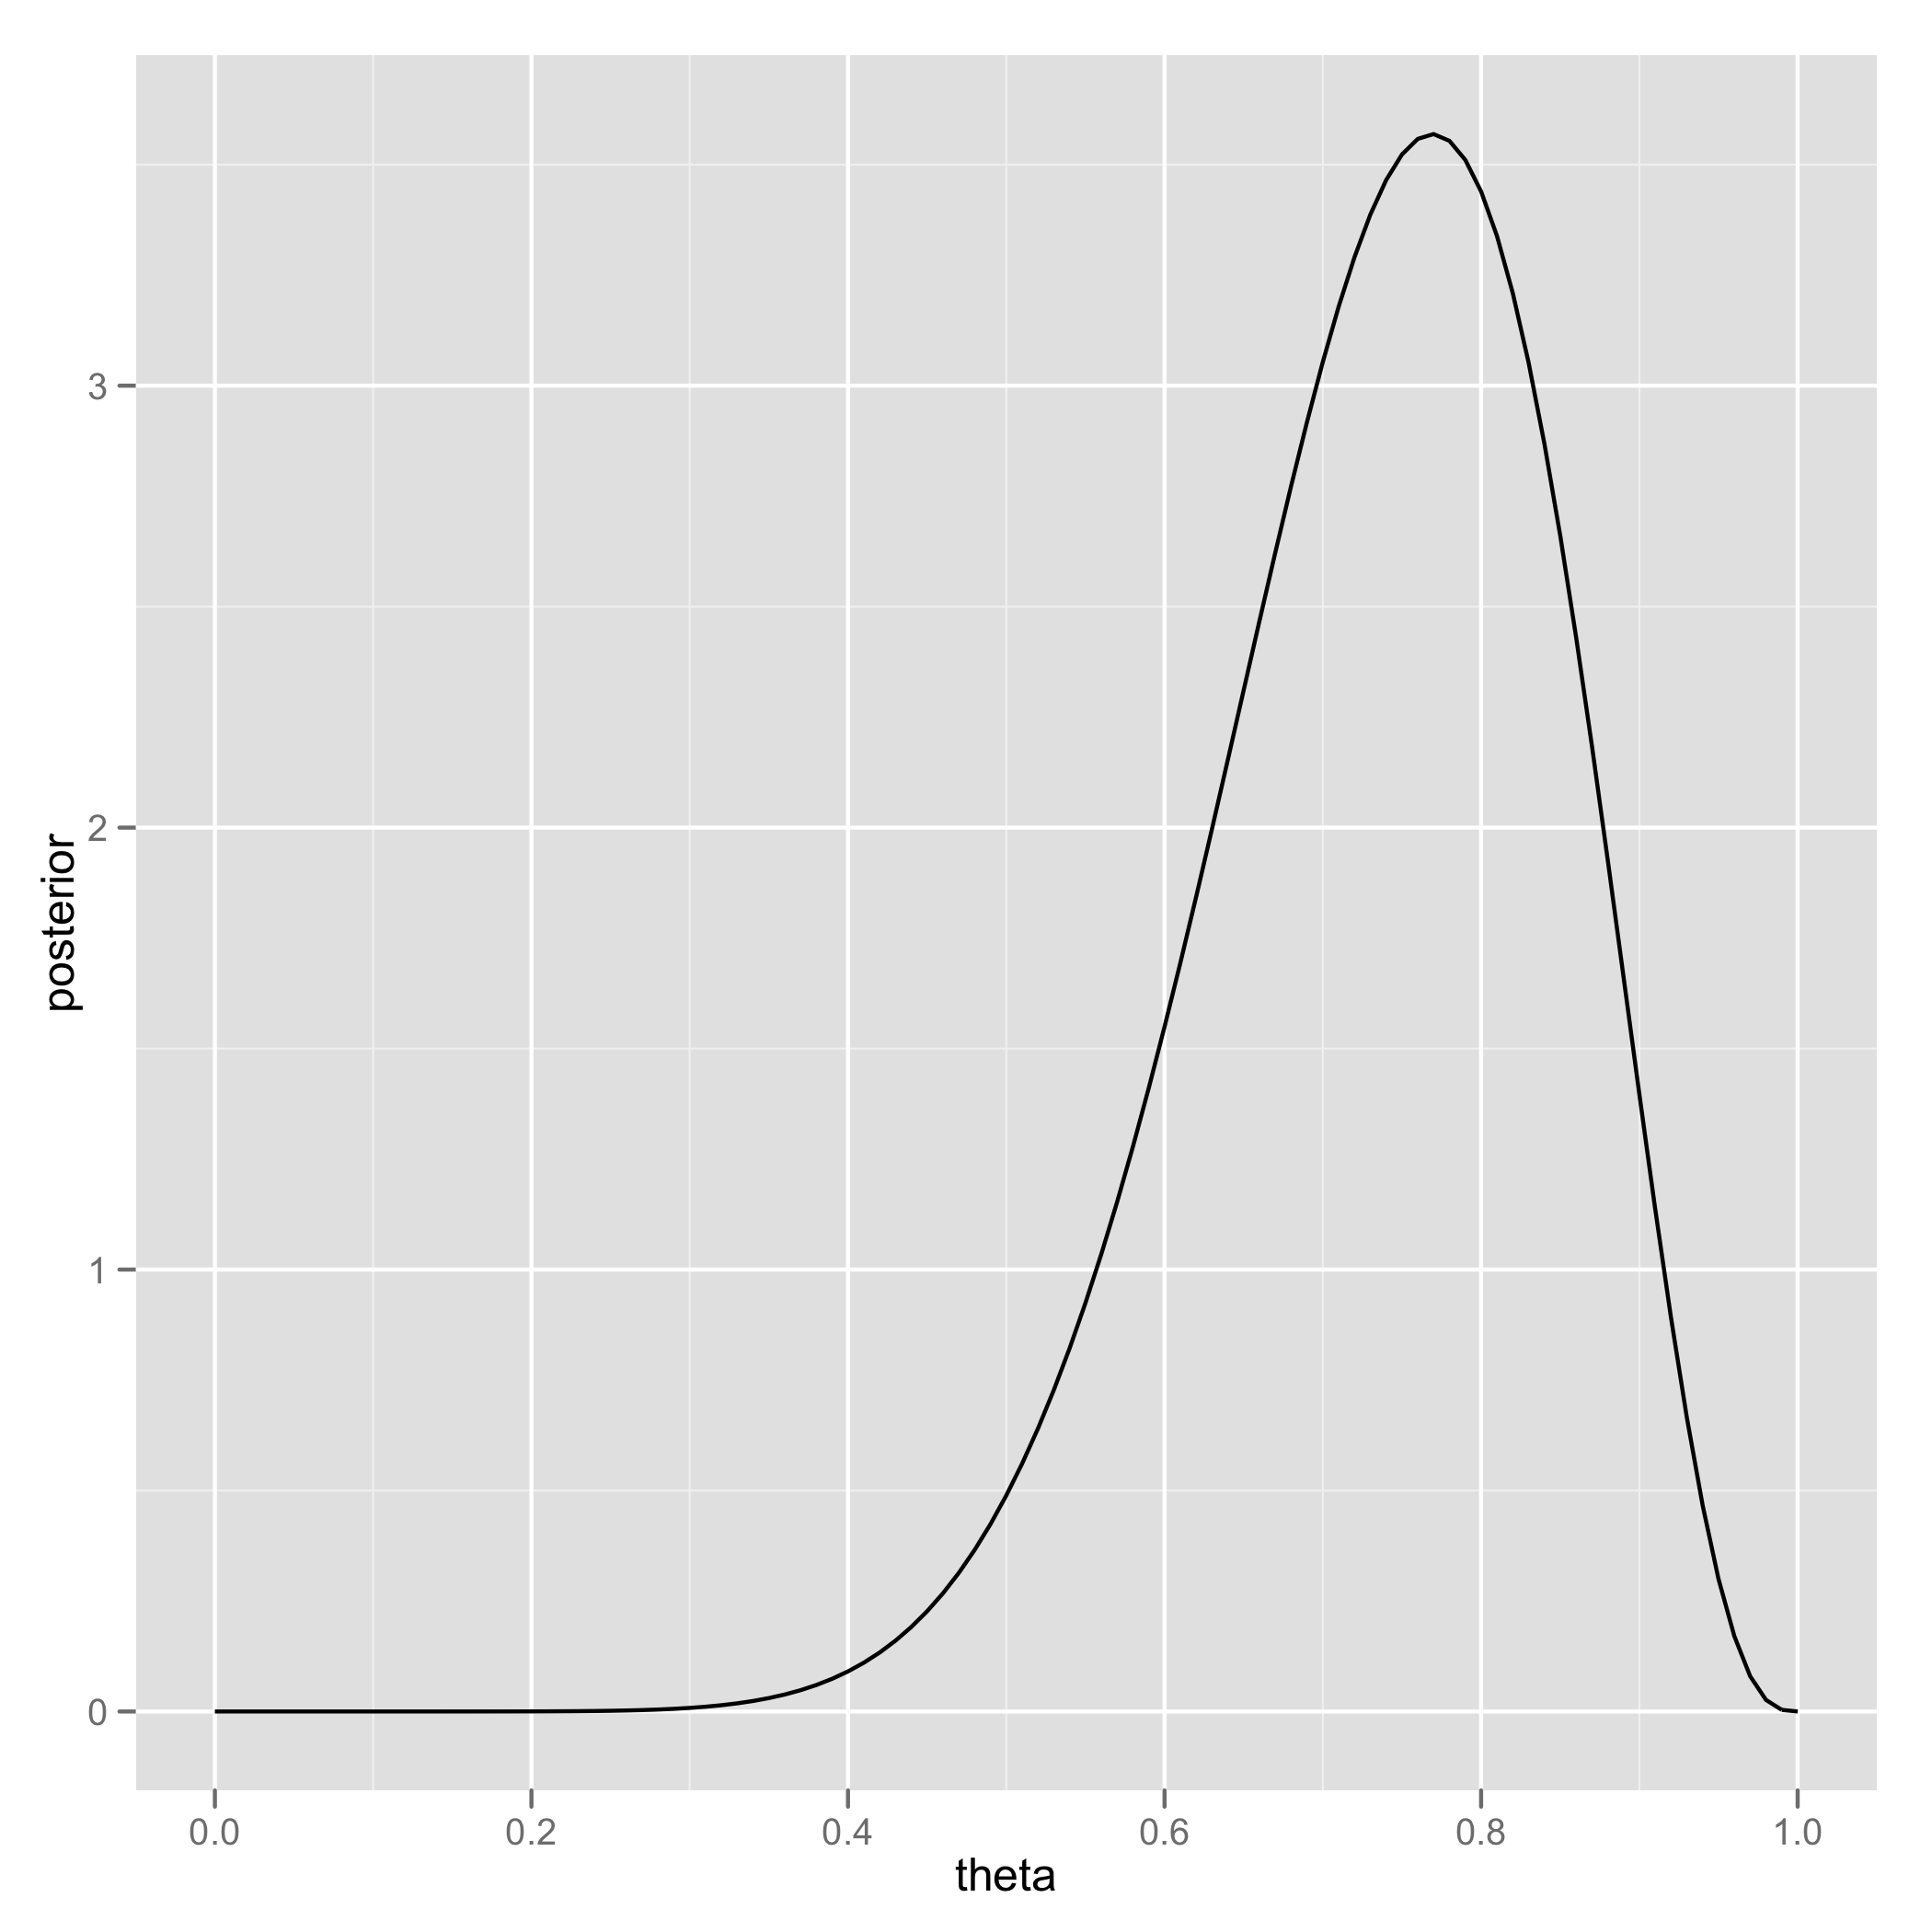
\includegraphics[scale = 0.1]{beta_distribution.png}
  \end{center}
}

\frame
{
  \begin{itemize}
    \item{Visualizing the full posterior can tell us a lot}
    \item{What other things can we do?}
  \end{itemize}
}

\frame
{
  \begin{itemize}
    \item{We can extract various point estimates from the posterior}
    \begin{itemize}
      \item{Means}
      \item{Medians}
      \item{Modes}
    \end{itemize}
    \item{We can compute interval estimates}
    \begin{itemize}
      \item{95\% probability intervals using quantiles}
    \end{itemize}
  \end{itemize}
}

\frame
{
  \begin{itemize}
    \item{When we use the mode of the posterior as our estimate we call it the MAP}
    \item{MAP stands for Maximum A Posteriori}
    \item{It is the Bayesian analogue to the MLE}
  \end{itemize}
}

\frame
{
Using the MAP via maximizing its log value is like penalized maximum likelihood:
\[
\log[p(\theta | D)] = \log[L(\theta | D) p(\theta)] = \log[L(\theta | D)] + \log[p(\theta)]
\]
}

\frame
{
\begin{itemize}
\item{Instead of finding the MAP, we can extract other values:}
\begin{itemize}
  \item{The mean of the posterior}
  \item{The median of the posterior}
  \item{Quantiles of the posterior}
\end{itemize}
\item{To decide which value to use, we can use decision theory}
\end{itemize}
}

\frame
{
  Decision theory:
  \begin{itemize}
    \item{We must decide what action to take}
    \item{We estimate the value of each action using our posterior}
    \item{We select the decision with the highest expected value}
  \end{itemize}
}

\frame
{
  Pascal's Wager:
  \begin{itemize}
    \item{Assume that our estimated probability that God exists is $p$}
    \item{Then the expected value of belief in God is $(1 - p) * 0 + p * \infty$}
    \item{The expected value of disbelief in God is $(1 - p) * 0 + p * 0$}
    \item{We should therefore choose to believe}
  \end{itemize}
}

\frame
{
  \begin{itemize}
    \item{In statistics, our decision is our estimate of $\theta$}
    \item{We choose the estimate that minimizes our expected loss}
  \end{itemize}
}

\frame
{
  \begin{itemize}
    \item{If the loss for an estimate $\hat{\theta}$ is $(\theta - \hat{\theta})^2$, the best estimate is the posterior mean}
    \item{If the loss for an estimate $\hat{\theta}$ is $|\theta - \hat{\theta}|$, the best estimate is the posterior median}
    \item{If the loss for an estimate $\hat{\theta}$ is $1$ if $\theta \neq \hat{\theta}$, the best estimate is the highest posterior mode}
  \end{itemize}
}

\frame
{
  \begin{itemize}
    \item{In practice, from now on, we're just going to use the mean and median of the posterior as point estimates}
  \end{itemize}
}

\begin{frame}
  \begin{itemize}
    \item{In modern Bayesian statistics, we use conjugacy whenever we can}
    \item{Otherwise, we use MCMC techniques}
  \end{itemize}
\end{frame}

\frame
{
  \begin{itemize}
    \item{MCMC depends on a remarkable result}
    \item{We can draw samples from a probability distribution that's known only up to a constant}
    \item{The posterior is just such a distribution}
    \item{The constant is the evidence}
  \end{itemize}
}

\begin{frame}
  \begin{itemize}
    \item{MCMC techniques draw many samples from the posterior}
    \item{There are therefore Monte Carlo methods}
    \item{As such, their quality increases when we take more samples}
    \item{To find each sample, a Markov chain is used}
    \item{Therefore MCMC $=$ Markov chain Monte Carlo methods}
  \end{itemize}
\end{frame}

\begin{frame}
  \begin{itemize}
    \item{For many problems, MCMC analysis can be completely automatic}
    \item{Part II of the seminar will work through many examples of applied Bayesian computation}
    \item{We'll use an MCMC tool called BUGS that fully automates MCMC sampling}
    \item{If you want to learn how MCMC works under the hood, there are many good books}
  \end{itemize}
\end{frame}

\end{document}
